\documentclass[12pt]{article}
\usepackage[margin=1in]{geometry}
\usepackage[backend=biber, style=numeric-comp, sorting=none]{biblatex}
\usepackage{graphicx}
\usepackage{float}	
\usepackage{hyperref}
\usepackage{enumitem}
\usepackage{rotating}
\addbibresource{references.bib}

\hypersetup{
    colorlinks,
    citecolor=black,
    filecolor=black,
    linkcolor=black,
    urlcolor=black
}

\makeatletter
\renewcommand\paragraph{\@startsection{paragraph}{4}{\z@}%
            {-3.25ex \@plus1ex \@minus.2ex}%
            {1.5ex \@plus.2ex}%
            {\normalfont\normalsize\bfseries}}
\makeatother
\setcounter{secnumdepth}{4}
\setcounter{tocdepth}{4}


\title{RISC-V: A Didactic Platform \\
Report}
\author{Jules PERRIN, Professor: Theo KLUTER}
\date{\today}

\begin{document}
\maketitle
\tableofcontents

\section{Introduction}
\subsection{Motivation}
This project, RISC-V: A Didactic Platform, embarks on the pursuit of simplifying complex computer architecture concepts, 
targeting an academic audience who is striving to comprehend the intricate world of processor design. 
It specifically focuses on the creation of a RV32I processor, based on the RISC-V instruction set architecture.

RISC-V, an open standard instruction set architecture (ISA), has increasingly gained popularity due to its simplified design and 
flexibility for customization. While its usage has been witnessed across a multitude of applications, its potential as an educational tool remains largely unexplored. 
The objective of this project is to bridge this gap by providing a detailed, comprehensible, and implementable design of an RV32IM processor, leveraging the RISC-V architecture.

This project not only contributes to the existing body of knowledge around RISC-V and processor design but also aims to democratize access to information on complex computing architectures. 
Through this platform, users will not only learn the theory behind processor design but will also gain valuable hands-on experience with the actual implementation, 
enabling them to better understand the interplay between hardware and software in a computing system.

In an era where the understanding of computer architecture is pivotal for both hardware and software development, 
a project like RISC-V: A Didactic Platform can serve as a crucial resource. 
By harnessing the power of the RISC-V architecture and presenting it through a user-friendly and accessible platform, 
we hope to elevate the understanding of processor design to new heights.
\subsection{Project Scope}
Here are the different main focus points of the project:


\begin{enumerate}[label={\textbullet}]
    \item Openess: It is an important point for the project to use as much as possible
    open source software and also for the project to be as open as possible such that people 
    can work on it with the less possible restrictions.
    \item Comprehensive: Since the project needs to be open source and be used by academic people
    to understand but also add things on top of it, the project needs to focus on being as comprehensive 
    as possible.
    \item Simplicity: This point is linked a bit with the last one, but the project doesn't aim as 
    performance first, but more as ease of understanding, so if a solution can be easier but degrade 
    a bit the performance, it should be taken except if it adds an educational value to do it
\end{enumerate}
\subsection{Project Objectives}

Overall, the project aims to give a very basic implementation of an RV32IM processor such 
that it can be used as an academic tool to teach and explain how a RISC processor works 
and how to build one using HDL languages such as Verilog. Here are the main objectives that 
has been set for the project:

\begin{enumerate}[label={\textbullet}]
    \item First create an unpipelined version of the RV32IM processor as a proof of concept
    \item Pipeline the existing unpipelined version of the processor
    \item Fix the different issues caused by the pipelining of the processor, mainly the 
    data dependency but also the branch prediction problem by either stall or implementing some 
    forwarding paths and branch predictor and mechanisms to make everything work correctly
    \item The simulation should works on Icarus Verilog to make the whole process more open instead 
    of relying on proprietary software such as Questa Modelsim.
    \item Add extensive testing of the different main modules to make the processor as reliable 
    as possible.
    \item Add an easy way for users to create programs and load them into the ROM memory.
    \item Document everything such that users can easily understand how things work and can 
    work on it easily.
\end{enumerate}

\section{Background Research and Knowledge}
\subsection{RISC-V}
RISC-V is an open-source instruction set architecture (ISA) based on the reduced instruction set
computer (RISC) principles. It is a free and open ISA enabling a new era of processor innovation
through open standard collaboration.

Most of the research I've done on it to understand how it works and how to implement it has been
done on the official website of the RISC-V foundation~\cite[p.~9-25]{riscv_manual} and of course more precisely
the chapter about the RV32I base integer instruction set. Inside it describes how the different instructions
are encoded with the 6 different formats~\cite[p.~104-105]{riscv_manual} that are used to encode the different instructions but also 
how the different instructions should behave using a mix of the manual but also a reference card~\cite[p.~81-83]{refcard}.
\subsection{Architecture}
\subsubsection{Unpipeline}
The unpipelined version of the CPU is mostly inspired by the one we did during the Comparch 1-2
courses at EPFL since NiosII and RISC-V are very similar. The main difference is that the RISC-V
is a 32 bits architecture while NiosII is a 16 bits architecture and also that RISC-V has a lot more
instructions than NiosII with small differences in how they work. 

\subsubsection{Pipeline}
The pipelined version is inspired also mostly by what we did during the Comparch 2 course at EPFL but
since we didn't implement the branch predictor and the forwarding paths, I had to imagine and think about 
most of the implementation myself. I've only done a couple of research to see if I could find some examples of 
such implementation mostly about forwarding paths since I wasn't sure how to implement it correctly at first 
glance. I've used mainly this pdf~\cite{forwarding_paths} to reassure myself that I was doing it correctly.
The branch predictor part has an algorithm I haven't invented called a two-level adaptive branch predictor~\cite{two_level_adaptive}.
It uses a 2 bits saturating counter but also knows patterns such that the predictions apply locally to the 
branch. It is a very simple algorithm but it works well enough for this project.
\subsection{Verilog}
Not knowing anything about Verilog since at EPFL we used VHDL instead, I had to learn it from scratch.
For that, I've used a website given by the professor~\cite{verilog_tutorial} that explains the basics of Verilog and how to use it.
From here I've started creating small modules and searching for examples on the internet to see how other people were doing it
and also when needed I've used different forums to find answers to my questions and when needed consulted the official 
Verilog documentation~\cite{verilog_doc}.
\subsection{Simulation Tools}
During the project, I mainly used a close source simulator that we were using at EPFL and 
developed by Intel called Questa Modelsim. It is a great tool combining compiling and seeing 
the waveforms of the signals in the same window. It is also very easy to use and has a lot of
features that I haven't used during the project. The only downside is that it is not free and
it is quite buggy sometimes and you need to activate an option called \texttt{full visibilty}
to have access to all the signals in the waveform window. At the end of the project, since I had 
to implement the CI, I needed a free simulator with a command line interface and I've used
Icarus Verilog. It is a free simulator that is not too hard to use and has a command-line interface.
The only downsides I've found while using it are that there is not a lot of documentation~\cite{icarus_tutorial} 
and it is a bit less user-friendly than Questa Modelsim. You have to use a different tool to see the waveforms
like GTKWave and you don't have access to the array of signals easily like in Questa Modelsim.
Also, one weird issue I've encountered is that the simulation gives different results than Questa Modelsim
because the full visibility option does things differently than Icarus Verilog, but I've luckily
found the issue even though to this day I don't know why it was doing that.
\subsection{RISC-V Toolchain}
\subsubsection{Developping using Assembly Code}
It is not that easy to find a way to compile a RISC-V RV32I assembly code into a hexadecimal file 
that can be read by the ROM module. So for that, I've found two projects that helped me 
develop simple programs for testing purposes. The first one is a Python script that converts
pseudo instructions into hexadecimal instructions~\cite{riscv_python_assembler}. The second one is a
website that converts assembly code into hexadecimal instructions~\cite{riscv_online_assembler}.
One last tool I've used to reverse the hexadecimal instructions into assembly code is a website~\cite{riscv_online_encoder_decoder} but 
also used it to modify one instruction at a time to see what it does.

\subsubsection{RISC-V GNU Compiler Toolchain}
The RISC-V GNU Compiler Toolchain is a set of tools that allows you to compile C/C++ code into
RISC-V assembly code. It is composed of a compiler, an assembler, a linker and a debugger. To use it 
you need to compile it from the source code which was not that easy to do because the documentation for
such a small architecture set is not that great and since we're developing bare metal programs, it is even
harder to find information about it. So I've used the official documentation~\cite{riscv_gnu_toolchain} and
also a tutorial I've found on the internet~\cite{riscv_gnu_toolchain_baremetal_tutorials} to compile it and finally use 
it.

\section{Design}
All the different constants were used in the project such that the different values linked to the different operators for 
the LSU, BRU and ALU. It is not an ideal solution but since Verilog doesn't have a better way to share 
constants by for example doing enums, I decided to do it this way. So all the constants are in the parameters.vh file inside 
the Verilog directory.
\subsection{Unpipelined Design}
The first step in the project other than learning how to develop in Verilog was to create an unpipelined version of the intended processor.
This version is quite more simple than the pipelined version as it doesn't have to deal with the hazards that can occur in a pipelined and 
issues with branches and jumps but also because it doesn't need any pipeline registers in between the different stages. I will give you an 
overall view of the design without the details of each connection between the different modules since it is not the main focus of this project 
and was more of a way to learn how to use Verilog and the tools associated with it but also a temporary step before the pipelined version.

\begin{figure}[H]
    \centering
    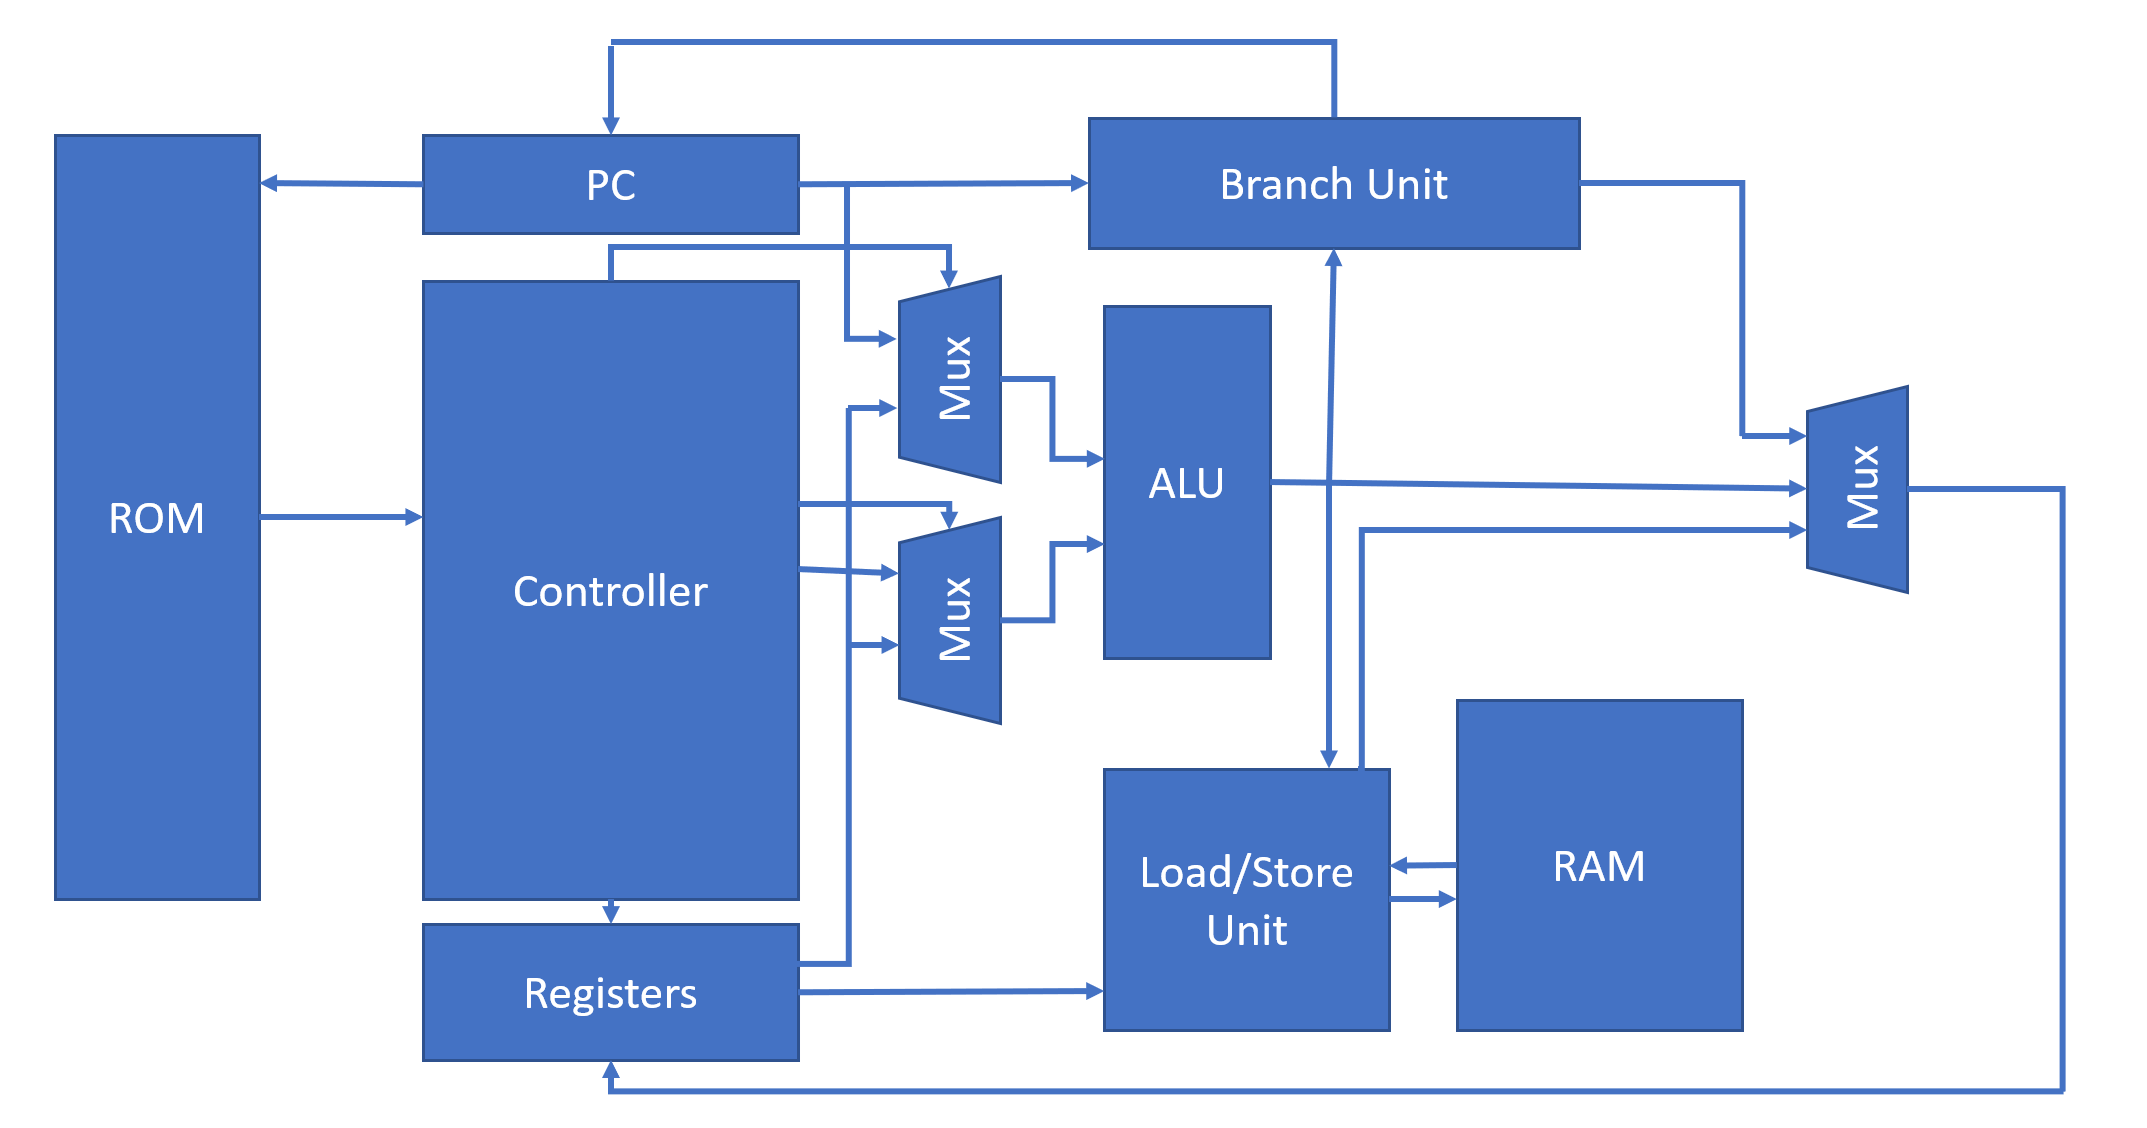
\includegraphics[width=0.85\textwidth]{design/unpipelined/images/unpipelined_cpu.png}
    \caption{Unpipelined CPU design}
    \label{fig:unpipelined_cpu_design}
\end{figure}

I will not go into the details of each module since it will be done in the next section about the pipelined version but I will give you a
brief overview of how the unpipelined version works.
First, the instruction is loaded from the ROM using the address given by the PC (Program Counter). Then the instruction needs to be decoded to know 
what it does and what are the operands and that's the job of the Controller that will try to match the different types of instruction to finally 
find the right one. Once it is done, it will output the different control signals to the register file, the ALU, the branch unit and the load/store unit such 
that it executes the instruction correctly with the correct data. The role of the ALU (Arithmetic Logic Unit) is to execute the different arithmetic
and logic operations such as addition, subtraction, multiplication, division, bitwise operations, etc. In the case of a branch instruction, the branch unit
will check if the instruction is a conditional one or not. In case it is one then it uses the result of the ALU to check if the condition is true or not
and update the PC accordingly. Finally, the load/store unit will load or store data from or to the RAM depending on the instruction. It is also using the 
result of the ALU since we can offset the address by an immediate value and that needs to be done by the ALU\@.
At the end of the cycle, a MUX will select among the three different results (ALU, branch unit and load/store unit) the one that will be written to the register file
according of course to the instruction executed.
Everything is done in one cycle and the next instruction is loaded from the ROM and the process starts again. \\

As we can see, the unpipelined version is quite simple then why do we need to pipeline it? The answer is performance. Indeed, the unpipelined version
is quite slow since it needs to wait for the instruction to be executed before loading the next one. But that can be improved by pipelining the processor
that will divide the execution of an instruction into multiple stages and execute multiple instructions at the same time and that's what we will see in the next section.


\subsection{Pipelined Design}
So what is the purpose of a Pipelined version of a CPU\@? As stated in the previous section, the unpipelined version is quite slow since it needs to wait for the instruction to be executed before loading the next one. 
Pipelining follows the idea of dividing the work among smaller parts and executing them in parallel. In the case of a CPU, it means that we will divide the execution of an instruction into multiple stages and execute multiple instructions at the same time.
Since each part has a smaller quantity of work to do, we can hopefully increase the clock frequency and thus obtaining in average a better throughput resulting in better performance.

\begin{figure}[H]
    \centering
    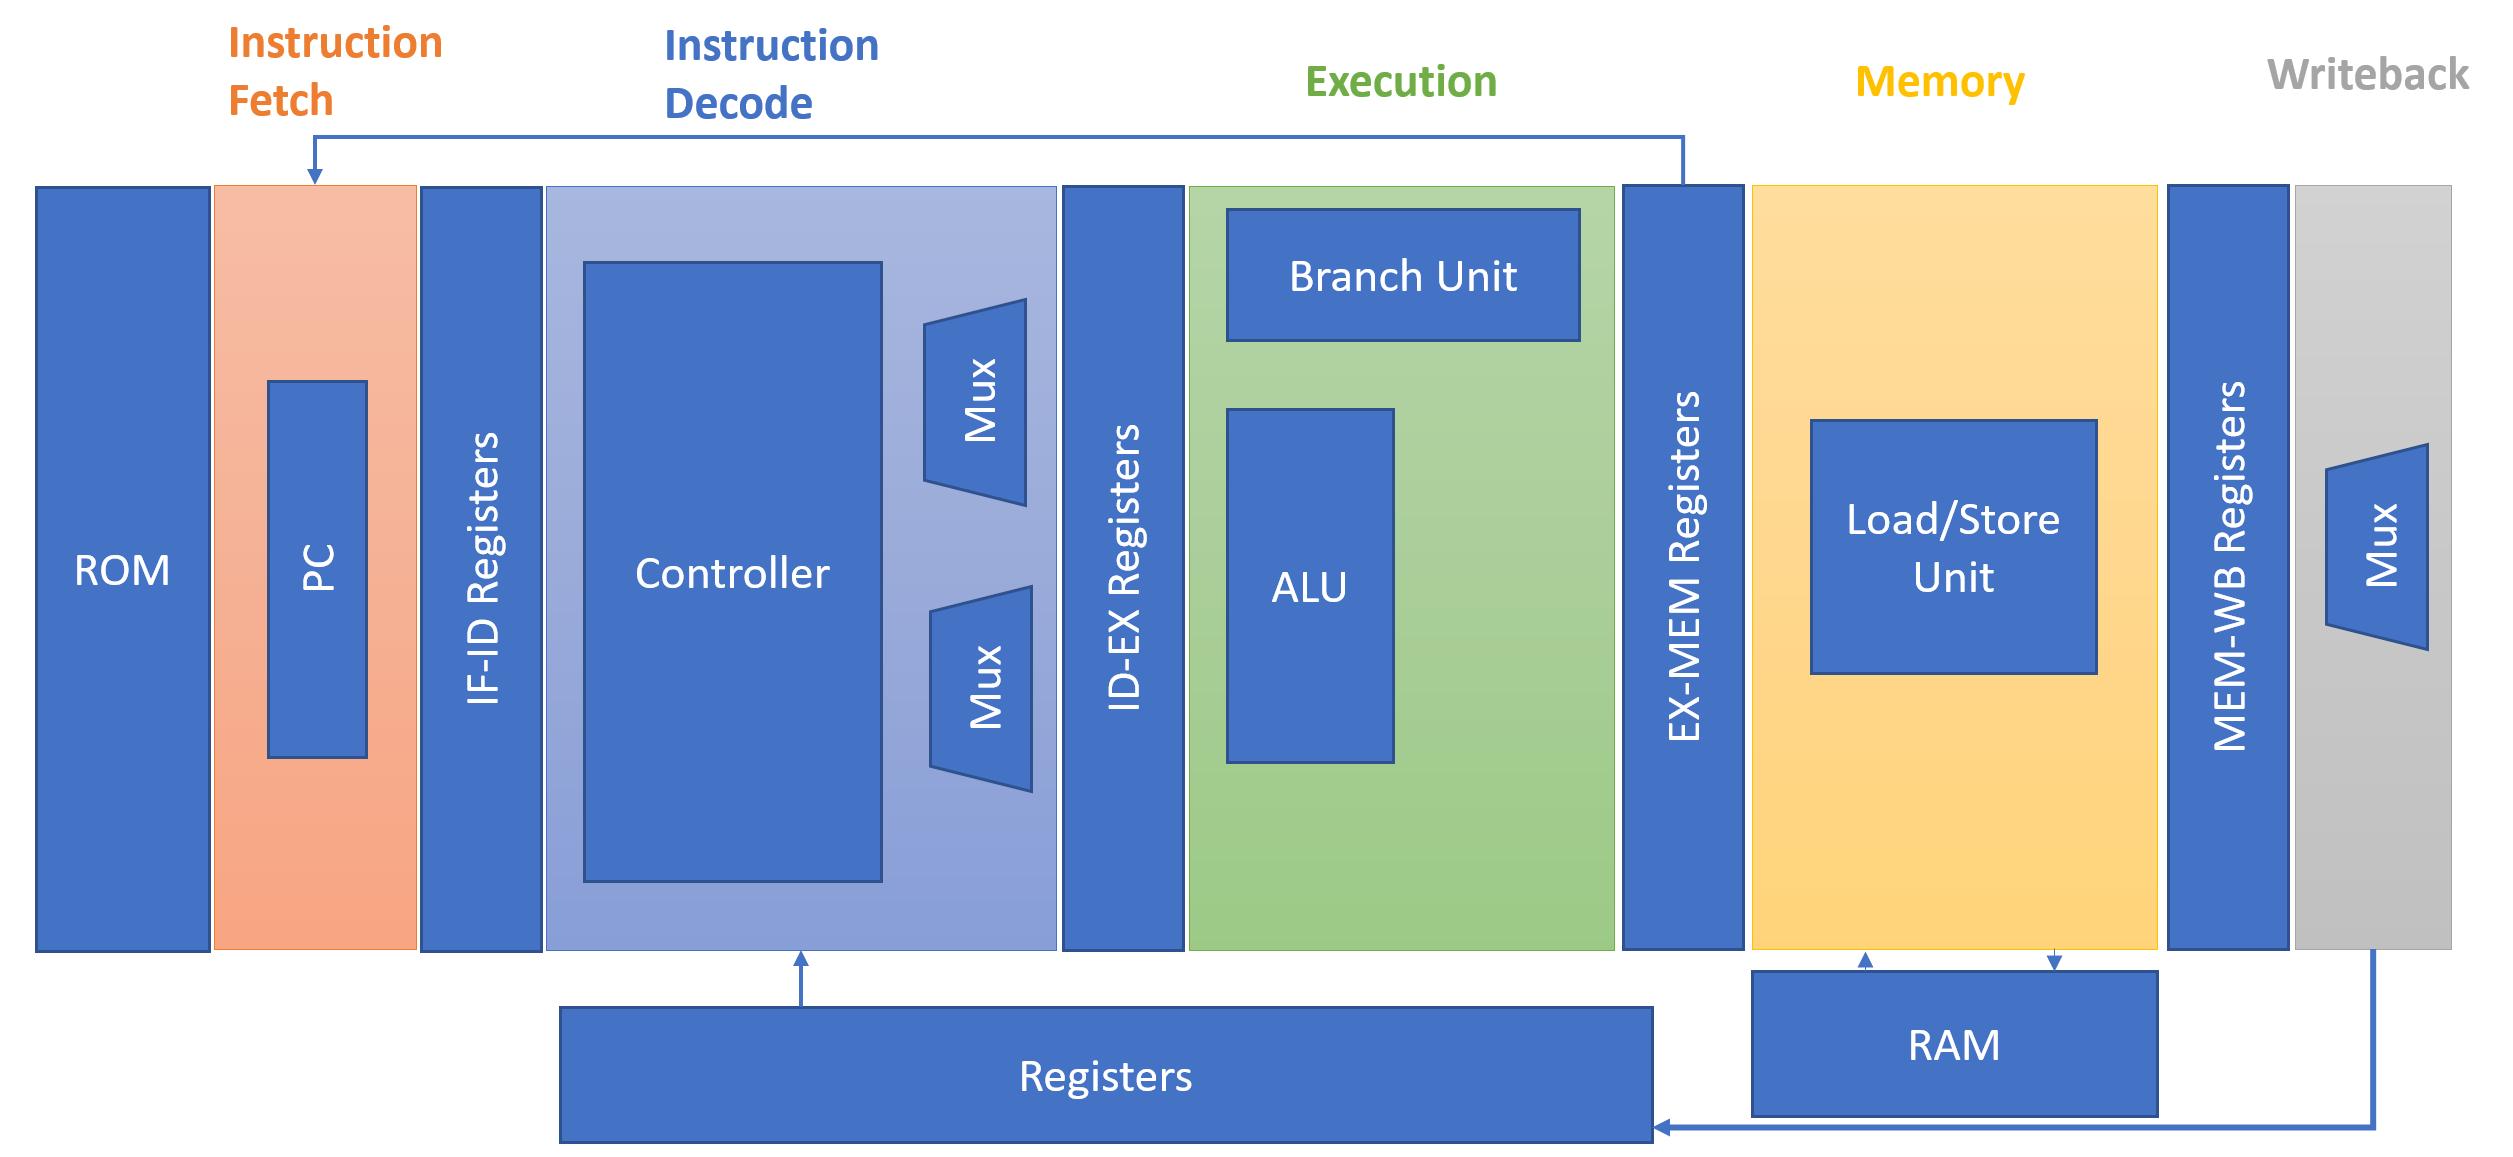
\includegraphics[width=1\textwidth]{design/pipelined/images/pipelined_design.png}
    \caption{Pipelined CPU design}
    \label{fig:pipelined_cpu_design}
\end{figure}

So here is the idea, we will divide the execution of instruction into five stages: Instruction Fetch (IF), Instruction Decode (ID), Execute (EX), Memory (MEM) and Write Back (WB).
Each stage will be executed in parallel and will be connected to the next one using pipeline registers. The pipeline registers are used to store the data between each stage and are synchronized with the clock.
The IF stage will fetch the instruction from the ROM using the PC (Program Counter) and will send it to the ID stage. The ID stage will decode the instruction and send the control signals to the different units 
(ALU, Branch Unit, Load/Store Unit) and will also send the operands to the EX stage. The EX stage will execute the instruction and send the result to the MEM stage. 
The MEM stage will load or store data from or to the RAM and send the result to the WB stage. Finally, the WB stage will write the result to the register file. \\

But for the most attentive reader or anybody with a bit of experience in computer architecture, you may have noticed that there is a problem with this design. 
This design will lead so some issues in two different ways. 

\begin{enumerate}[label=\textbullet]
    \item The first one is that since instruction is not executed anymore in one cycle, its result will not be available in the next cycle.
    This is an issue because if the next instruction depends on the result of the previous one, it will not be able to execute correctly and will use 
    outdated data from the registers. This is called a \textbf{Data Hazard}.
    \item The second one is related to the branching mechanism, since the result of the branch will be available only after the EX stage, the PC will not be updated
    before that leading to possible wrong instructions being fetched and executed in the pipeline. This is called a \textbf{Control Hazard}.
\end{enumerate}

For resolving these two issues we have two solutions. Either stalling the pipeline when a hazard is occurring or when a branch is detected at the IF stage such that we wait for 
the result before fetching any new instruction. One issue with this approach is of course performance which is unfortunate since the main purpose of pipelining is to improve performance.

Another solution for the data hazard is to use \textbf{Forwarding} which consists of forwarding the result of the ALU to the EX stage and the result of the MEM stage to the EX and MEM stages.
The only moment we will have to stall the pipeline is when we have a load instruction followed by an instruction using the result of the load. In this case, we will have to stall the pipeline
for one cycle to wait for the result of the load.

\begin{figure}[H]
    \centering
    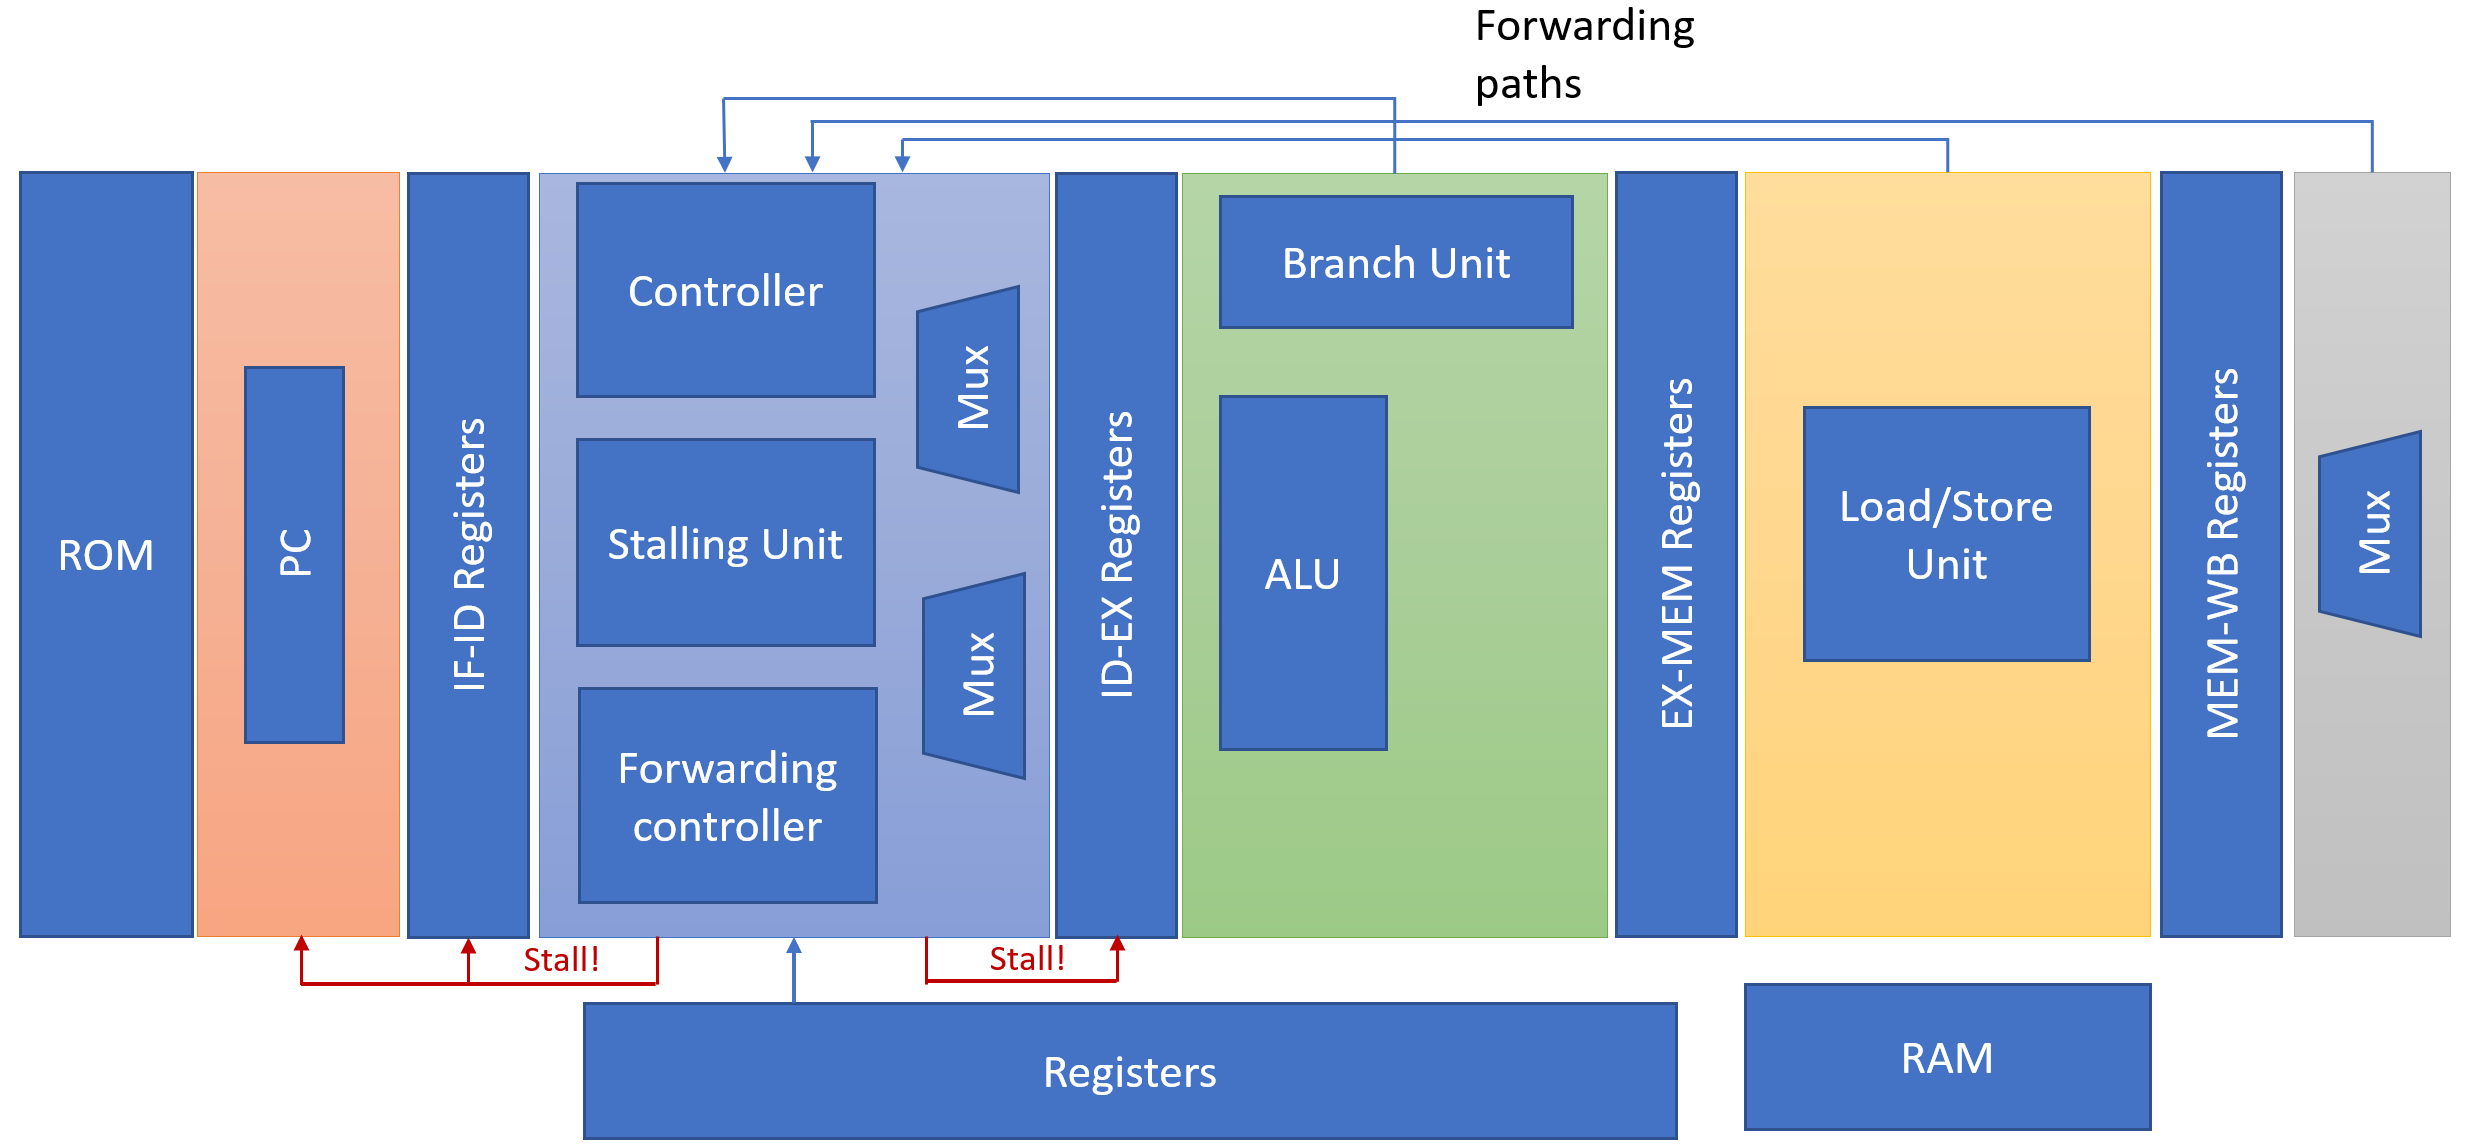
\includegraphics[width=1\textwidth]{design/pipelined/images/pipelined_design_forwarding.png}
    \caption{Pipelined CPU design with forwarding paths}
    \label{fig:pipelined_cpu_design_forwarding}
\end{figure}

Another solution for the control hazard is to use \textbf{Branch Prediction} which consists of predicting the result of the branch and fetching the instruction at the predicted address.
It is not always possible to predict correctly the result of a branch but it is possible to use some heuristics to improve the prediction accuracy. For example, we can predict that a branch will not be taken
if the previous branch was not taken. This is called a \textbf{Branch Not Taken} heuristic. Another heuristic is to predict that a branch will be taken if the previous branch was taken. This is called a \textbf{Branch Taken} heuristic.
Of course, you can develop more complex heuristics but this is out of the scope of this project and I invite you to use the link in the reference to the given algorithm I've chosen 
to implement in the CPU\@. But when the prediction is wrong, we will have to flush the pipeline and restart the execution from the correct address. \\

\begin{figure}[H]
    \centering
    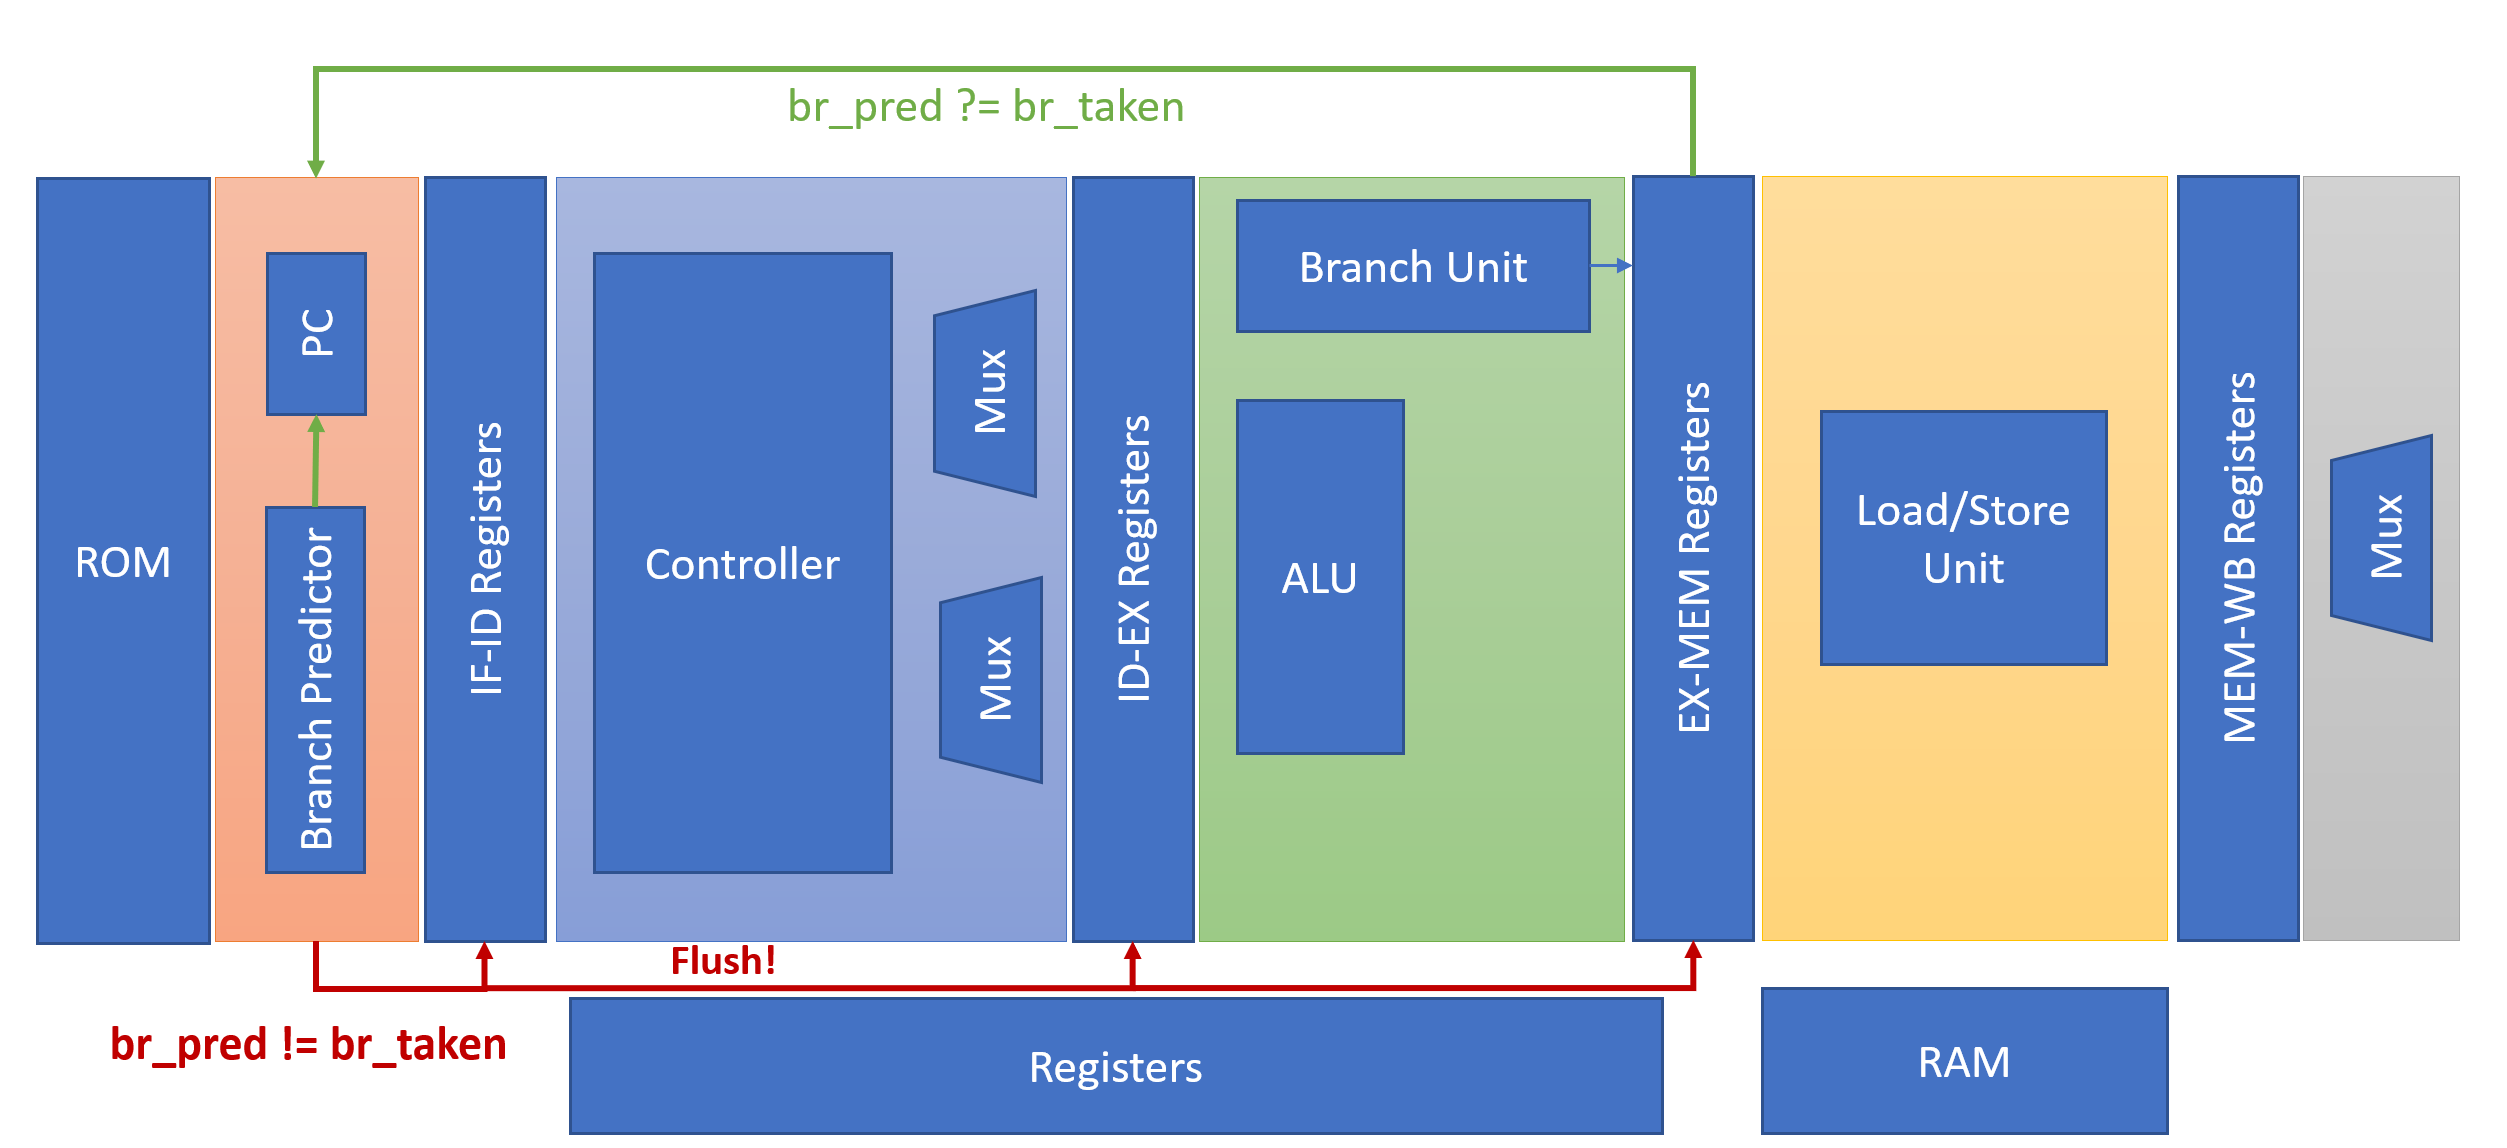
\includegraphics[width=1\textwidth]{design/pipelined/images/pipelined_design_predictor.png}
    \caption{Pipelined CPU design with branch predictor}
    \label{fig:pipelined_cpu_design_predictor}
\end{figure} 

Now we can see the full simplified representation of the pipelined CPU design. 
\begin{figure}[H]
    \centering
    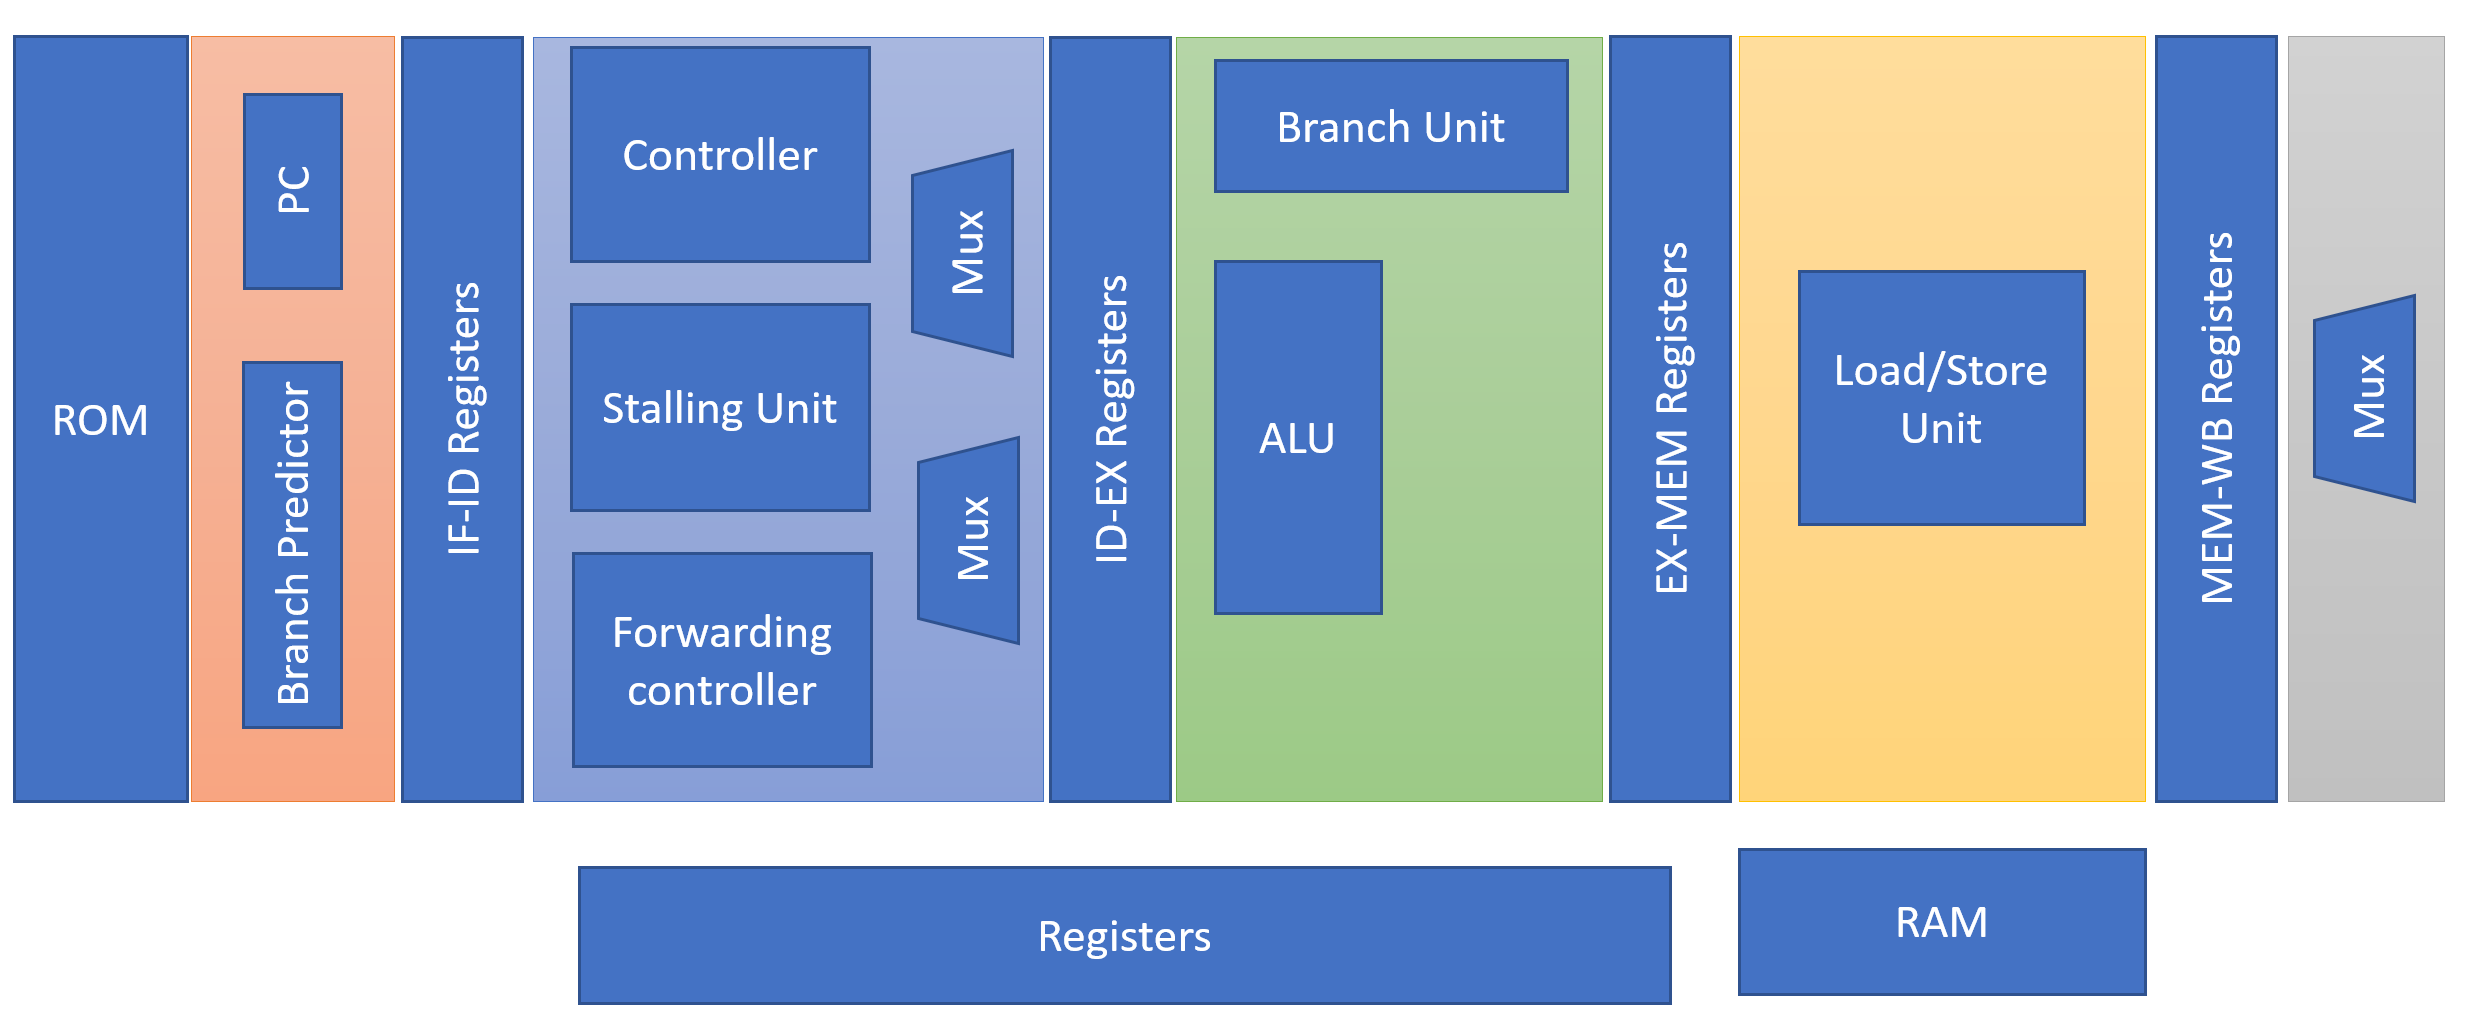
\includegraphics[width=1\textwidth]{design/pipelined/images/pipelined_design_full.png}
    \caption{Pipelined CPU simplified design with forwarding paths and branch predictor}
    \label{fig:pipelined_cpu_design_full}
\end{figure}

A more detailed version with all the different signals and how they are connected is available in the appendix \ref{appendix:pipelined_design} and
also as a diagram inside the project \texttt{diagrams} folder that can be opened \href{https://app.diagrams.net/}{here}. \\

Now that we have a better understanding of the overall design, I can go into more detail about each different stage and the modules inside of them.

\subsubsection{IF Stage}
\subsection{PC}

\begin{figure}[H]
\centering
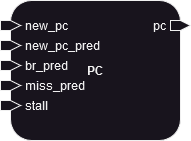
\includegraphics[width=0.5\textwidth]{../diagrams/fetch/pc.png}
\caption{Diagram of the PC}
\label{fig:PC}
\end{figure}

The PC is responsible for computing the next PC. It uses the different input signals to know which PC to compute.
for example, if it is a branch, the branch predictor will tell him what to do, and if the branch predictor is wrong
it will be updated accordingly. If it is a more classic instruction such as an ADD, it will simply increment the PC by 4
etc. \\

Signals:
\begin{enumerate}
    \item Input: $new\_pc$, This signal represent the next PC given by the branch unit in the EX stage.
    \item Input: $new\_pc\_pred$, This signal represent the next PC given by the branch predictor.
    \item Input: $br\_pred$, This signal is representing the state of the prediction made by the branch predictor in the EX stage.
    \item Input: $miss\_pred$, This signal is representing if there is a miss prediction or not.
    \item Input: $stall$, This signal is representing if the pipeline is stalled or not due to a data dependency in the ID stage.
    \item Output: $pc$, This signal is representing the current PC.
\end{enumerate}
\subsection{Branch Predictor}

\begin{figure}[H]
\centering
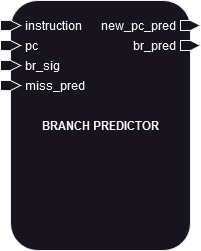
\includegraphics[width=0.5\textwidth]{../diagrams/fetch/br_predictor.png}
\caption{Diagram of the Branch Predictor}
\label{fig:br_predictor}
\end{figure}

The branch predictor as its name suggests is responsible for predicting if the branch will be taken or not. The algorithm that 
is being used is the two-level adaptive branch predictor, which I will not describe in detail but reuse the idea of a 
2-bit saturating counter but apply a bit of the notion of locality and pattern recognition. Of course, the algorithm
could be improved or replaced by any other algorithm and it is up to the user to do it if he wants to.
It works at the beginning by doing a simple matching on the current instruction to see if it is a branch instruction.
If that's the case we look if it is a conditional branch or not, if it is not we simply predict that the branch will be taken for 
the JAL instruction, but the JALR one will be always predicted as not taken for data dependency reasons. If it is a conditional branch
we simply use the algorithm described above to predict if the branch will be taken or not. The algorithm updates the prediction depending 
on the actual result of the branch that is represented by the $miss\_pred$ signal. If the prediction is taken, we compute the next PC \\

Signals:
\begin{enumerate}[label={\textbullet}]
    \item Input: $instruction$, This signal is representing the current instruction that is being fetched.
    \item Input: $pc$, This signal is representing the current PC.
    \item Input: $br\_sig$ This signal is representing the state of the current instruction in the EX stage. It is used to know if the instruction is a branch or not.
    such that it updates only the algorithm when it is a branch instruction.
    \item Input: $miss\_pred$, This signal is representing the state of the prediction made by the branch predictor in the EX stage.
    \item Output: $new\_pc\_pred$, This signal is representing the next PC that will be used if the prediction is taken.
    \item Output: $br\_pred$, This signal is indicating if the branch is predicted as taken or not.
\end{enumerate}


\subsubsection{ID Stage}
\subsection{Controller}

\begin{figure}[H]
\centering
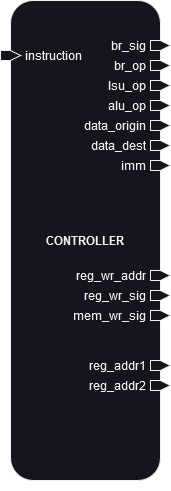
\includegraphics[width=0.35\textwidth]{../diagrams/decode/controller.png}
\caption{Diagram of the Controller}
\label{fig:controller}
\end{figure}

The controller is the main module of the ID stage. It is responsible for decoding the current instruction which is the action
of extracting the different fields of the instruction and forwarding them to the next stage. For more information about the different
types of instruction and how the data is encoded in the instruction, please refer to the RISC-V manual~\cite{riscv_manual}. \\

Signals:
\begin{enumerate}
    \item Input: $instruction$, This signal is representing the current instruction that is being decoded.
    \item Output: $br\_sig$, This signal is representing the state of the current instruction. 
    It is used to know if the instruction is a branch or not.
    \item Output: $br\_op$, This signal is representing the type of branch that is being executed.
    \item Output: $lsu_op$, This signal is representing the type of load or store that is being executed.
    \item Output: $alu\_op$, This signal is representing the type of ALU operation that is being executed.
    \item Output: $data\_origin$, This signal is representing the origin of the data that is being used by the ALU.
    That could be the registers, or one register and an immediate or one register and the PC.
    \item Output: $data\_dest$, This signal will be useful in the write-back stage to know which data to write back,
    so either the ALU result or the data from the memory or the next PC (so the PC+4).
    \item Output: $imm$, This signal is representing the immediate value that is being used by the ALU.
    \item Output: $reg\_wr\_addr$, This signal is representing the register address that will be written back.
    \item Output: $reg\_wr\_sig$, This signal is representing if we want to write to the register file or not.
    \item Output: $mem\_wr\_sig$, This signal is representing if we want to write to the memory or not.
    \item Output: $reg\_addr1$, This signal is representing the first register address that has been extracted from the instruction.
    \item Output: $reg\_addr2$, This signal is representing the second register address that has been extracted from the instruction.
\end{enumerate}
\subsection{Forward Controller}

\begin{figure}[H]
\centering
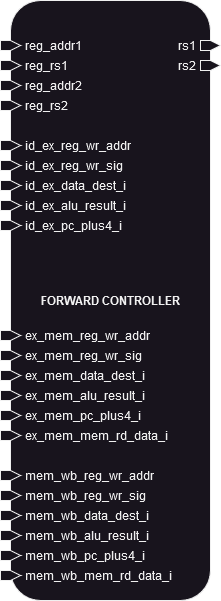
\includegraphics[width=0.35\textwidth]{../diagrams/decode/forward_controller.png}
\caption{Diagram of the Forward Controller}
\label{fig:forward_controller}
\end{figure}

The forward controller is a module that is used to control what are the values used as rs1 and rs2 in the ALU. 
For example, if you have a data dependency between two instructions, the first one is a load and the second one is an add,
you need to forward the result of the load to the ALU. This module is responsible for that and instead of using the value of the register file,
it will use the value that is being forwarded. \\

Signals:
\begin{enumerate}[label={\textbullet}]
    \item Input: $reg_addr1$, This signal is representing the first register address that is being used by the current instruction.
    \item Input: $reg_rs1$, This signal is representing the value of the first register that is being used by the current instruction.
    \item Input: $reg_addr2$, This signal is representing the second register address that is being used by the current instruction.
    \item Input: $reg_rs2$, This signal is representing the value of the second register that is being used by the current instruction.
    \item Input: $id\_ex\_reg\_wr\_addr$, This signal is representing the register address that is being written by the previous instruction.
    \item Input: $id\_ex\_reg\_wr\_sig$, This signal is representing if the previous instruction is written to the register file or not.
    \item Input: $id\_ex\_data\_dest$, This signal is representing the origin of the data that is being used by the ALU in the previous instruction.
    \item Input: $id\_ex\_alu\_result$, This signal is representing the result of the ALU in the previous instruction.
    \item Input: $id\_ex\_pc\_plus4$, This signal is representing the pc plus 4 of the previous instruction.
    \item Input: $ex\_mem\_reg\_wr\_addr$, This signal is representing the register address that is being written by the previous instruction.
    \item Input: $ex\_mem\_reg\_wr\_sig$, This signal is representing if the previous instruction is written to the register file or not.
    \item Input: $ex\_mem\_data\_dest$, This signal is representing the origin of the data that is being used by the ALU in the previous instruction.
    \item Input: $ex\_mem\_alu\_result$, This signal is representing the result of the ALU in the previous instruction.
    \item Input: $ex\_mem\_pc\_plus4$, This signal is representing the pc plus 4 of the previous instruction.
    \item Input: $ex\_mem\_mem\_rd\_data$, This signal is representing the data that is being read from the memory in the previous instruction.
    \item Input: $mem\_wb\_reg\_wr\_addr$, This signal is representing the register address that is being written by the previous instruction.
    \item Input: $mem\_wb\_reg\_wr\_sig$, This signal is representing if the previous instruction is written to the register file or not.
    \item Input: $mem\_wb\_data\_dest$, This signal is representing the origin of the data that is being used by the ALU in the previous instruction.
    \item Input: $mem\_wb\_alu\_result$, This signal is representing the result of the ALU in the previous instruction.
    \item Input: $mem\_wb\_pc\_plus4$, This signal is representing the pc plus 4 of the previous instruction.
    \item Input: $mem\_wb\_mem\_rd\_data$, This signal is representing the data that is being read from the memory in the previous instruction.
    \item Output: $rs1$, This signal is representing the value that should be used as rs1 in the ALU.
    \item Output: $rs2$, This signal is representing the value that should be used as rs2 in the ALU.
\end{enumerate}
\paragraph{Stall Unit}

\begin{figure}[H]
    \centering
    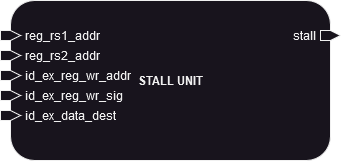
\includegraphics[width=0.5\textwidth]{design/pipelined/decode/images/stall_unit.png}
    \caption{Diagram of the Stall Unit}
    \label{fig:stall_unit}
\end{figure}

The stall unit is a small module that is used to stall the pipeline when a data dependency that cannot be resolved by forwarding is detected
which should only happen if we use the result of a load instruction in the next instruction. It is simply comparing the register addresses of the
current instruction with the register that is being written by the previous instruction. If there is a match, it looks what is the operation that is
being executed by the current instruction and if it is a load, it will stall the pipeline. \\

Signals:
\begin{enumerate}[label={\textbullet}]
    \item Input: $reg\_rs1\_addr$, This signal is representing the first register address that is being used by the current instruction.
    \item Input: $reg\_rs2\_addr$, This signal is representing the second register address that is being used by the current instruction.
    \item Input: $id\_ex\_reg\_wr\_addr$, This signal is representing the register address that is being written by the previous instruction.
    \item Input: $id\_ex\_reg\_wr\_sig$, This signal is representing if the previous instruction is written to the register file or not.
    It is used to differentiate between a load and a store.
    \item Input: $id\_ex\_data\_dest$, This signal is representing the origin of the data that is being used by the ALU in the previous instruction.
    In this case only if the previous instruction has a data dest of MEM then we need to stall the pipeline.
    \item Output: $stall$, This signal is representing if we need to stall the pipeline or not.
\end{enumerate}
\paragraph{Mux}

\begin{figure}[H]
    \centering
    
\includegraphics[width=0.20\textwidth]{design/pipelined/decode/images/mux2.png}
    \caption{Diagram of the 2 entries Mux}
    \label{fig:mux2}
\end{figure}

The mux is a small module that is used to select between the two inputs that it has. It is used 2 times in this module, for selecting between
$rs1$ and $PC$ and for selecting between $rs2$ and $imm$. Sorry, I haven't used the standard shape of a MUX but I haven't found one on the 
website I'm using to draw the different diagrams. \\

Signals:
\begin{enumerate}[label={\textbullet}]
    \item Input: $a$, This signal is representing the first input of the mux.
    \item Input: $b$, This signal is representing the second input of the mux.
    \item Input: $sel$, This signal is representing the select signal of the mux.
    \item Output: $out$, This signal is representing the output of the mux.
\end{enumerate}

\subsubsection{EX Stage}
\subsection{ALU}

\begin{figure}[H]
\centering
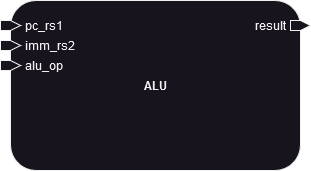
\includegraphics[width=0.75\textwidth]{../diagrams/execute/alu.png}
\caption{Diagram of the ALU}
\label{fig:alu}
\end{figure}

The ALU is a module that is responsible for executing the arithmetic and logic operations. So every mathematical operation is done in this module.

Signals:
\begin{enumerate}[label={\textbullet}]
    \item Input: $a$, This signal is representing the first input of the ALU.
    \item Input: $b$, This signal is representing the second input of the ALU.
    \item Input: $op$, This signal is representing the operation that the ALU will execute.
    \item Output: $out$, This signal is representing the output of the ALU.
\end{enumerate}
\subsection{Branch Unit}

\begin{figure}[H]
\centering
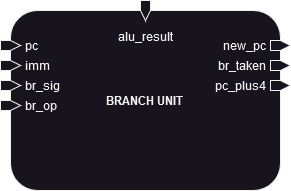
\includegraphics[width=0.5\textwidth]{../diagrams/execute/br_unit.png}
\caption{Diagram of the Branch Unit}
\label{fig:br_unit}
\end{figure}

The Branch Unit is a module that is responsible for computing the next PC. It is used in the EX stage. It uses the result of the ALU
for conditional branching to know if the branch should be taken or not.

Signals:
\begin{enumerate}[label={\textbullet}]
    \item Input: $alu\_result$, This signal is representing the result of the ALU. Used for conditional branching.
    \item Input: $pc$, This signal is representing the current PC.
    \item Input: $imm$, This signal is representing the immediate value of the instruction. It is used as an offset for the branch.
    \item Input: $branch\_sig$, This signal mark if the instruction is a branch or not.
    \item Input: $br\_op$, This signal is representing the branch operation like for example BEQ, BNE etc.
    \item Output: $new\_pc$, This signal is representing the new PC computed by the branch unit.
    \item Output: $pc\_plus\_four$, This signal is representing the PC + 4. Used to save the value of the next instruction 
    to come back at it after a branch occurred.
    \item Output: $br\_taken$, This signal is representing if the branch is taken or not. Used in the IF stage to compare 
    to the branch predictor and know if the pipeline needs to be flushed or not.
\end{enumerate}

\subsubsection{MEM Stage}
\subsection{Load Store Unit}

\begin{figure}[H]
    \centering
    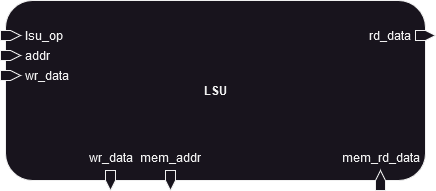
\includegraphics[width=0.5\textwidth]{../diagrams/memory/lsu.png}
    \caption{Load Store Unit}
    \label{fig:lsu}
\end{figure}

The LSU is a module that is responsible for memory access. It will manage the different READ and WRITE to the memory and for example
mask the data you want to read or write according to the given instruction.

Signals:
\begin{enumerate}[label={\textbullet}]
    \item Input: $lsu\_op$, This signal is representing the type of memory access you want to perform.
    \item Input: $addr$, This signal is representing the address of the memory you want to access.
    \item Input: $wr\_data$, This signal is representing the data you want to write to the memory.
    \item Input: $mem\_rd\_data$, This signal is representing the value that has been read from the memory.
    \item Output: $wr\_data$, This signal is representing the value that should be written to the memory and correctly
    masked according to the given instruction.
    \item Output: $mem\_addr$, This signal is representing the address you want to write or read to the memory.
    \item Output: $rd\_data$, This signal represents the value that has been read from the memory and correctly 
    masked according to the given instruction.
\end{enumerate}

\subsubsection{WB Stage}
\paragraph{Mux}

\begin{figure}[H]
    \centering
    
\includegraphics[width=0.20\textwidth]{design/pipelined/decode/images/mux2.png}
    \caption{Diagram of the 2 entries Mux}
    \label{fig:mux2}
\end{figure}

The mux is a small module that is used to select between the two inputs that it has. It is used 2 times in this module, for selecting between
$rs1$ and $PC$ and for selecting between $rs2$ and $imm$. Sorry, I haven't used the standard shape of a MUX but I haven't found one on the 
website I'm using to draw the different diagrams. \\

Signals:
\begin{enumerate}[label={\textbullet}]
    \item Input: $a$, This signal is representing the first input of the mux.
    \item Input: $b$, This signal is representing the second input of the mux.
    \item Input: $sel$, This signal is representing the select signal of the mux.
    \item Output: $out$, This signal is representing the output of the mux.
\end{enumerate}

\subsubsection{Pipeline Registers}
\begin{figure}[H]
    \centering
    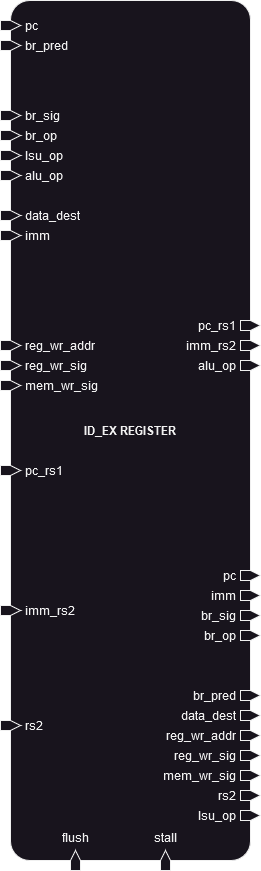
\includegraphics[width=0.35\textwidth]{design/pipelined/pipeline/images/pipeline.png}
    \caption{ID-EX Pipeline register example}
    \label{fig:pipeline}
\end{figure}

I will not explain the 4 different pipeline register stages in detail, and I will mainly describe as an example the 
pipeline between the ID Stage and the Ex Stage. The role of a pipeline register is to store the data that will be
passed to the next stage at each clock cycle such that you can increase throughput by increasing the clock frequency since 
you've divided the overall work in smaller chunks so you can do it in less time (theoretically).
What is also interesting here is the $stall$ and $flush$ signals. The first one is used to stop updating the pipeline when 
a data dependency is encountered. The second one is used when the branch predictor did a bad guess. In this case we need to 
flush the register that has incorrect instructions stored in them and instead just fill them with something similar to a NOP 
instruction.

\subsubsection{ROM, RAM and Register File}
\subsection{ROM}

\begin{figure}[H]
    \centering
    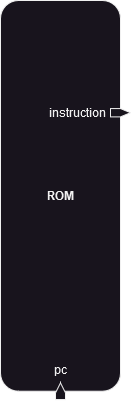
\includegraphics[width=0.35\textwidth]{../diagrams/rom_ram_reg/rom.png}
    \caption{ROM}
    \label{fig:rom}
\end{figure}

The ROM is responsible for storing the program that is being executed by the processor. As its name indicate, it is 
a read-only memory and for the moment it is capable of storing up-to 1024 instructions.

Signals:
\begin{enumerate}[label={\textbullet}]
    \item Input: $pc$, This signal gives the address that needs to be read in the memory.
    \item Output: $instruction$, This signal is representing the instruction that has been read from the ROM.
\end{enumerate}
\paragraph{RAM}

\begin{figure}[H]
    \centering
    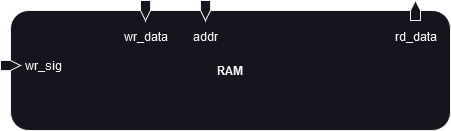
\includegraphics[width=0.5\textwidth]{design/pipelined/rom_ram_reg/images/ram.png}
    \caption{RAM}
    \label{fig:ram}
\end{figure}

The RAM is the main memory of the CPU, it can be used to store and read values. In this project, the RAM is also 1024 words long
and each word is 32 bits long.

Signals:
\begin{enumerate}[label={\textbullet}]
    \item Input: $addr$, This signal gives the address that needs to be read or written in the memory.
    \item Input: $wr\_sig$, This signal indicates if the given address need to be written or read
    \item Input: $wr\_data$, This signal gives the data that needs to be written in the memory.
    \item Output: $rd\_data$, This signal is representing the data that has been read from the RAM.
\end{enumerate}
\paragraph{Register File}

\begin{figure}[H]
    \centering
    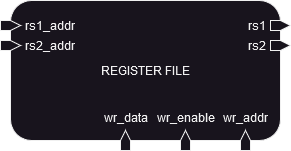
\includegraphics[width=0.5\textwidth]{design/pipelined/rom_ram_reg/images/register_file.png}
    \caption{Register File}
    \label{fig:register_file}
\end{figure}

The register file is a one-cycle really small memory. The RV32I standard requires 32 registers, each 32 bits long. Only the first (zero) register
has a given value of 0, the other can be used at will but as with any other architecture there are some standards for what a register is being used 
for.

Signals:
\begin{enumerate}[label={\textbullet}]
    \item Input: $rs1\_addr$, This signal gives the address of the first register that needs to be read.
    \item Input: $rs2\_addr$, This signal gives the address of the second register that needs to be read.
    \item Input: $wr\_addr$, This signal gives the address of the register that needs to be written.
    \item Input: $wr\_data$, This signal gives the data that needs to be written in the memory.
    \item Input: $wr\_enable$, This signal indicates whether the register should be written with the $wr\_data$ value.
    \item Output: $rs1$, This signal gives the value read at address $rs1\_addr$.
    \item Output: $rs2$, This signal gives the value read at address $rs2\_addr$.
\end{enumerate}










\section{Testing}
\subsection{Testbenches}

Some testbenches have been written for the biggest modules of the project. The only notable exception is the 
controller for time but also since it is mostly tested by the general CPU testbench. So here is the testbench that has been written:

\begin{enumerate}[label={\textbullet}]
    \item ALU
    \item Branch Unit
    \item CPU
    \item Forward controller
    \item LSU
    \item PC
    \item Register File
    \item Stall Unit
\end{enumerate}

Most of this testbench is testing the module with a lot of different (mostly random) inputs and checking that the output is correct.
Some are also testing more specific cases like corner cases that could lead to some issues in the design. The testbench for the CPU is 
a bit special since it is testing the whole CPU with a simple program computing a recursive sum of the first 10 integers testing most 
of the module of the CPU.
When writing the test I discovered some issues in the design, mostly in the ALU and the Branch Unit. For in the ALU I was shifting 
not correctly in one of my instructions, and in the Branch Unit the output of the alu wasn't treated as a signed number.
It's also with the CPU testbench that I've discovered the issue with the different values between Questa Modelsim with full visibility and 
Icarus Verilog. 
I maintain that we could enhance the range of our testing by incorporating additional checks across various testbenches, such as designing 
a program for the CPU that utilizes each of its unique instructions. Nevertheless, I believe that our current testing approach is reasonably satisfactory. \\

The process of actually launching the test and seeing the output has been simplified by me by creating a Makefile that will compile all the 
different modules correctly and link them together and it will launch the simulation and output the results into the terminal. Also, each 
testbench will generate a .vcd file that can be opened with GTKWave to see the different signals of the simulation. It is important to have
Icarus Verilog for that part to work since it doesn't use any containers that could improve portability but I think it's not needed 
in my opinion but that could be a nice improvement.

\begin{figure}[H]
    \centering
    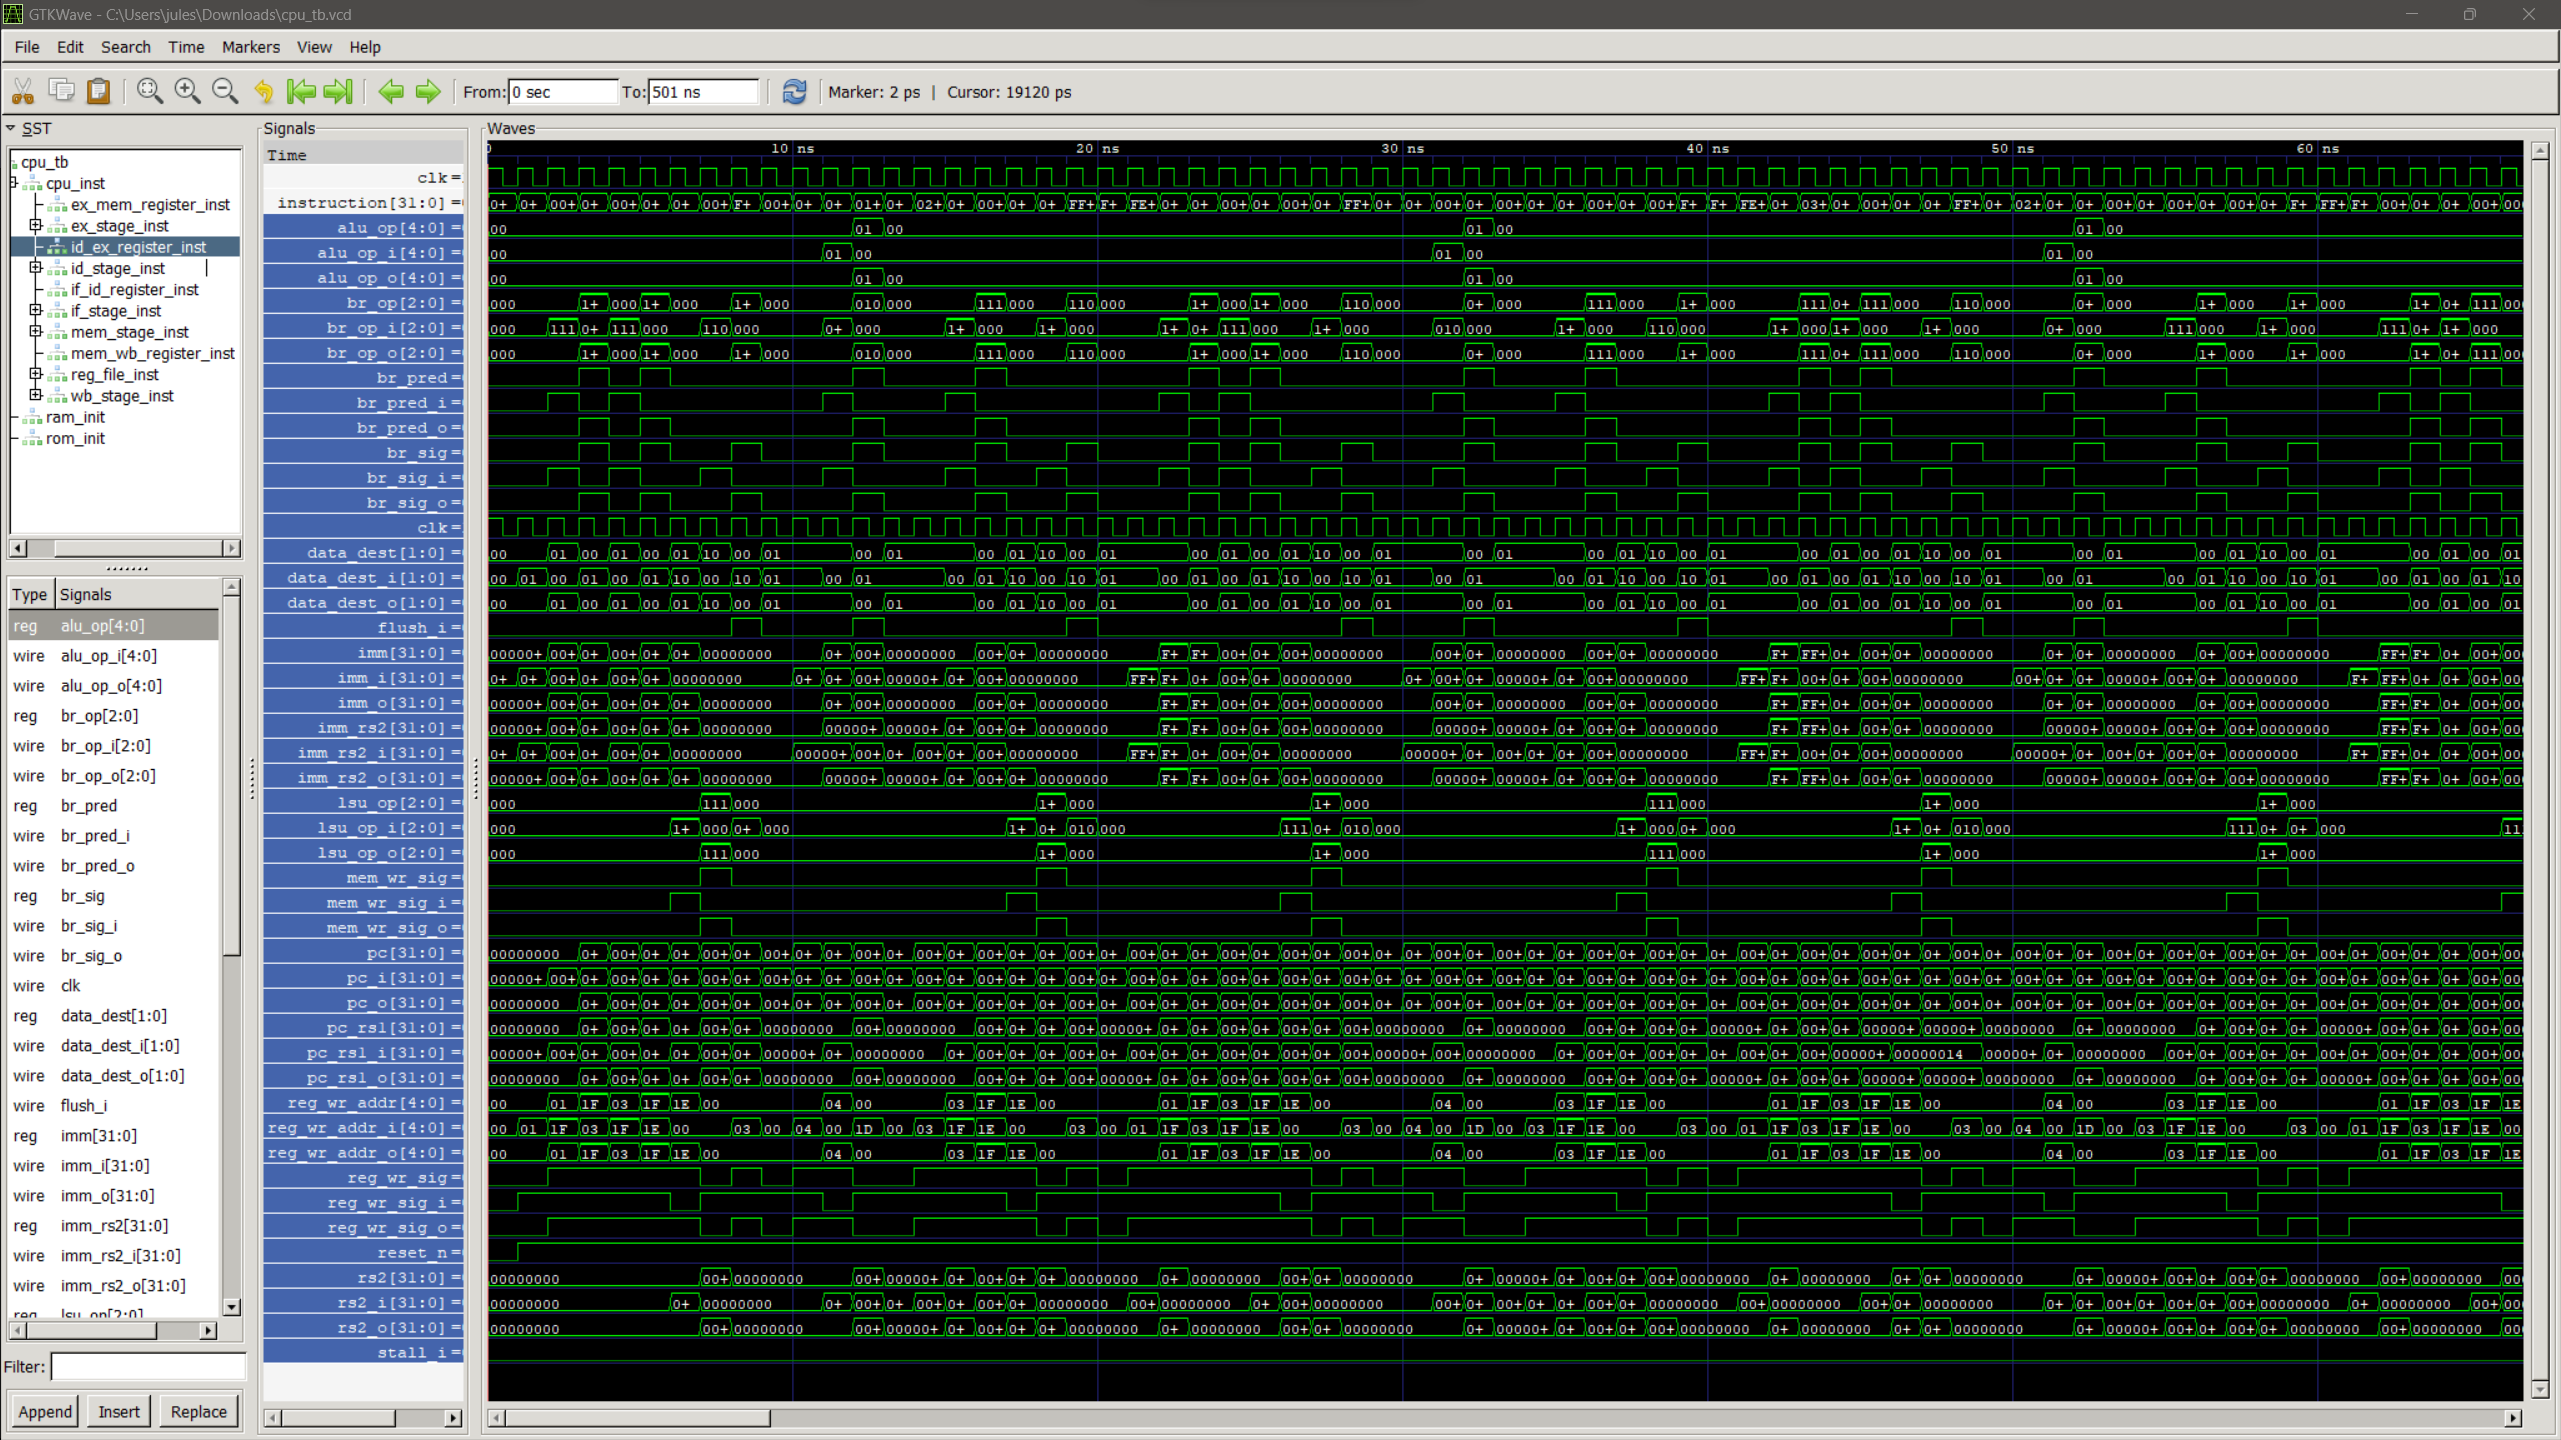
\includegraphics[width=1\textwidth]{testing/images/gtkwave.png}
    \caption{GTKWave output of the CPU testbench}
    \label{fig:gtkwave}
\end{figure}


\subsection{Continuous Integration}

The continuous integration is done with Cirrus CI. It is a free service for open-source projects that allows you to run tests on different
platforms. It is configured with a .cirrus.yml file at the root of the project. It works mostly like the local Makefile I've made to run 
the tests locally, but it uses the fact that failing test output a message with "FAIL" inside of them to detect if it should indicate that 
the running tests have failed or not. It also uses the fact that the testbench generates a .vcd file to upload it as an artifact of the build
so that you can download it and see the different signals of the simulation which can be helpful to debug the different issues.

\begin{figure}[H]
    \centering
    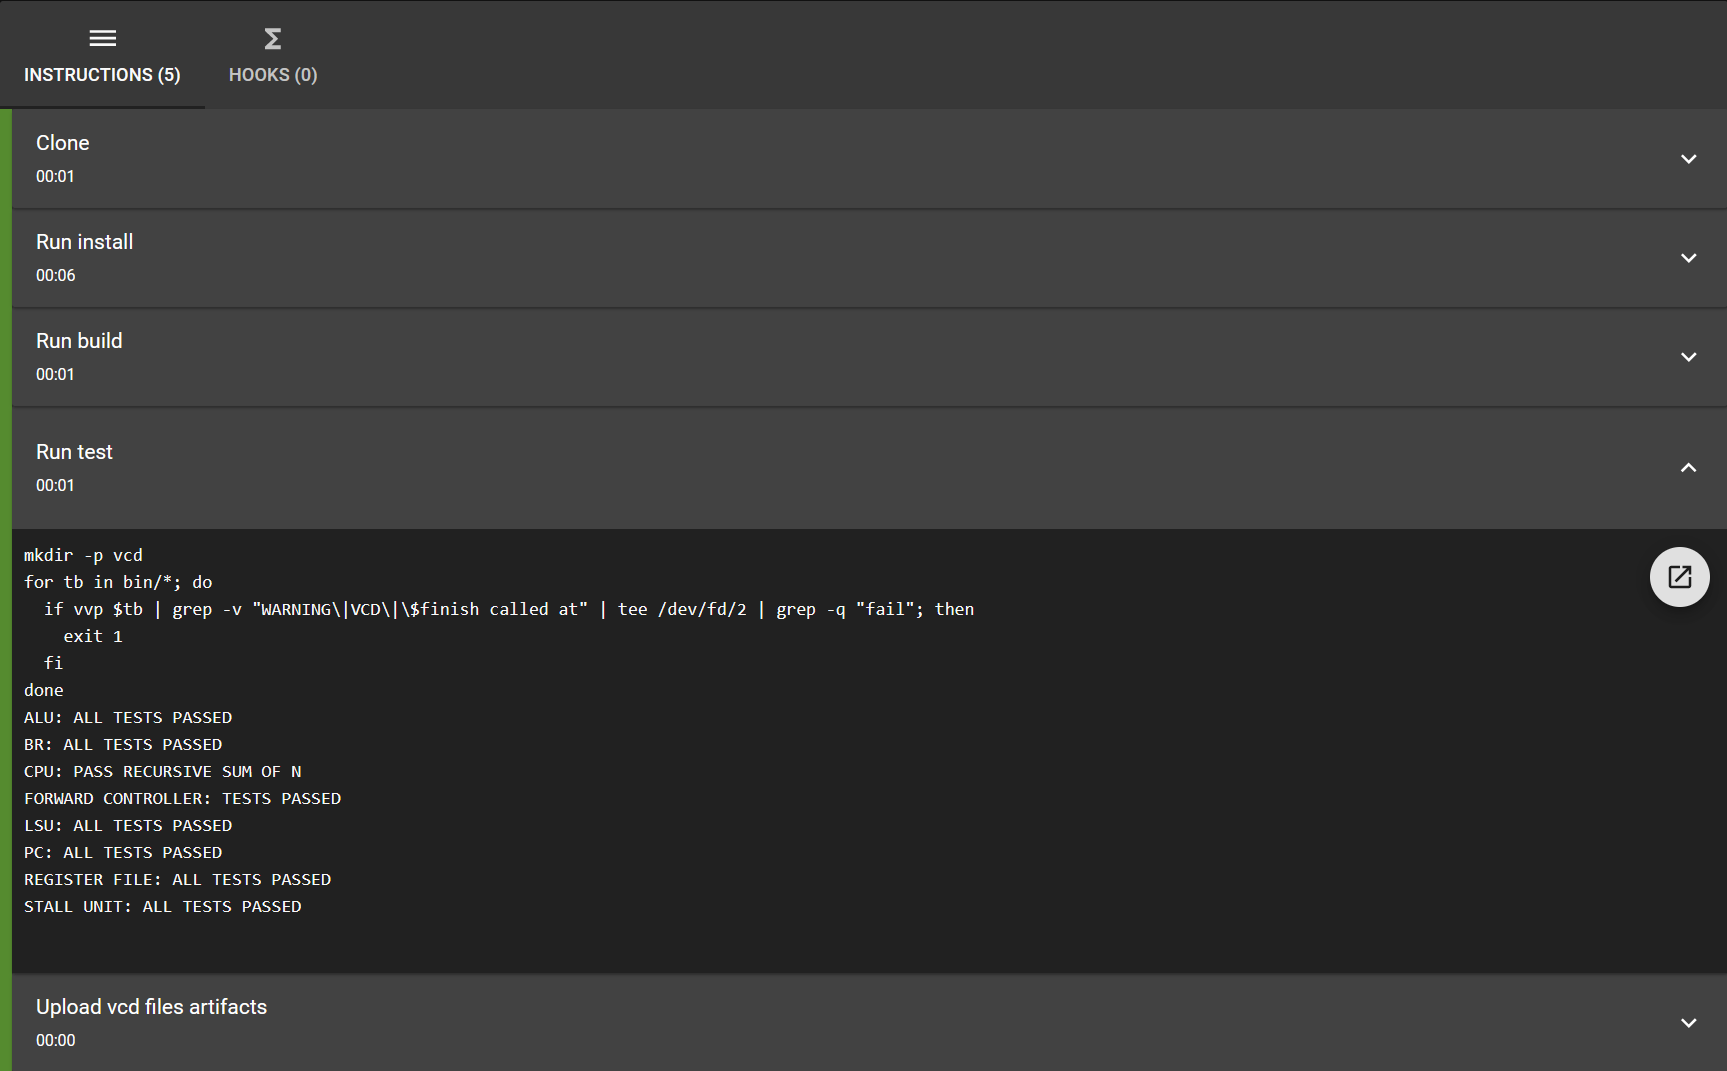
\includegraphics[width=1\textwidth]{testing/images/ci.png}
    \caption{Cirrus CI output after a commit}
    \label{fig:ci}
\end{figure}

The configuration was quite simple but I had issues after 2 weeks of using it where the docker image I was using wasn't working anymore for 
no apparent reason. So I've decided to simply use an Ubuntu environment and install the different dependencies manually. It's not a big 
deal since I've not a lot of dependencies and it's not taking a lot of time to install them. But it's still a bit annoying to have to
to pull the dependencies for each build instead of simply caching the build docker image. But it's still working fine and I'm happy with it.

\section{Developing programs for the CPU}
There are two main ways of developing programs for my CPU that I've set up.\\

The first one is using assembly code or pseudo assembly code and using this website\cite{riscv_online_assembler} and it will output 
the result in hexadecimal that is readable by the ROM, and the same for the python script\cite{riscv_python_assembler} but it uses a 
different syntax that is very close to actual RISC-V assembly.\\

The second one is using C code inside the \texttt{c\_code} folder of the project. But this solution requires a bit more work before 
using it since you have to compile the RISC-V toolchain with the correct architecture, so here RV32IM, then correctly give the variables 
to your bash environment and then you can compile the C code using the Makefile inside the \texttt{c\_code} folder. Here a detailed guide 
that combines the document from the RISC-V toolchain\cite{riscv_gnu_toolchain} and the tutorial I've found about bare metal RISC-V development
\cite{riscv_gnu_toolchain_baremetal_tutorials}.

\begin{enumerate}[label={\textbullet}]
    \item Clone the toolchain from \href{https://github.com/riscv-collab/riscv-gnu-toolchain}{here}.
    
    \begin{verbatim}
    git clone https://github.com/riscv/riscv-gnu-toolchain.git
    \end{verbatim}
    
    \item Navigate into the cloned directory.
    
    \begin{verbatim}
    cd riscv-gnu-toolchain
    \end{verbatim}
    
    \item Run the configuration script.

    \begin{verbatim}
    ./configure --prefix=/opt/riscv --with-arch=rv32im
    \end{verbatim}
    
    \item Compile the toolchain. This step may take a while.
    
    \begin{verbatim}
    make
    \end{verbatim}
    
    \item Once the compilation is done, add the toolchain to your PATH in your bash configuration file.

    \begin{verbatim}
    echo 'export PATH=$PATH:/opt/riscv/bin' >> ~/.bashrc
    source ~/.bashrc
    \end{verbatim}
\end{enumerate}

After that, you should be able to use the toolchain. To test it, you can try making a simple program like the ones in the 
$c\_code$ folder of the project. You can simply compile them with the following command:

\begin{verbatim}
    make
\end{verbatim}


The only thing that was needed after that to execute the C code is creating a linker file that indicates to the compiler where 
to put the different sections of the code and it has been done by me to facilitate the process and was quite simple to do actually.
The only "issue" you'll have is that since the architecture RV32IM is so small, the C standard library is not included in the toolchain
and you'll have to implement it yourself if you want to use it but I still think it is less painful than using assembly code.\\

\section{Conclusion}
Overall I'm really proud of what I've made during this semester on the project and don't regret at all going for this project.
I've learned and relearned a lot of things about computer architecture that will for sure consolidate my knowledge for the future
since I think I'll be working in this field. 
I've also learned a lot about the RISC-V architecture and how to implement it in Verilog and I think it is a really good architecture 
to learn about computer architecture since it is really simple and easy to understand.
I still think RISC-V is at the beginning of its life and will be a really good alternative to ARM in the future since it is open-source
but some of the tools to develop on it are still not as good as the other architectures and I've encountered some documentation issue 
during the project and finding some information was sometimes harder than it should have been.
I loved the autonomy and freedom that Professor Kluter gave me during the project and it corresponded more to my way of working
than some other projects, I've done during my studies. I think the time I spent on it was around the time I'd planned so I'm quite happy
that the project didn't take the time I should have dedicated to other courses.\\

What should be improved in the future?
I think the project is a really good start for a RISC-V processor but here is what I think can be added or improved in the project: 
\begin{enumerate}[label=\textbullet]
    \item Adding more extensions from the RISC-V ISA like the floating-point extension for example and could be a great starting
    point for any student that would like to continue the project.
    \item As said in the testing section, I think some testbenches could be improved and some more can be added to test the processor
    to make sure it is bug-free since I can't be 100\% sure that the processor is bug-free but most of the tests I've done manually
    and with the testbenches have passed so I think it is a least in a pretty good state.
    \item Maybe implement a memory hierarchy with a cache and a memory controller to make the processor more realistic.
    \item Trying to make a multi-core processor such that the FENCE instructions can be implemented and that could be a great
    way to link the BA5 course Mularch.
    \item Implementing a reordering of instructions to make the processor more efficient for example if the memory hierarchy is
    implemented, it will optimize the time spent waiting for the memory by executing other instructions.
    \item Create a simple interactive program that could be executed on the FPGA board using the processor like the snake game 
    we did in the Comparch course.
\end{enumerate}

Thank you again to Professor Kluter for allowing me to work on this project and for some of the resources he gave me 
to help me during the project. I hope this project will be useful for future students and that it will be improved in the future.
I hope you enjoyed reading this report and that it will help you understand the project better.

Of course, the project is accessible on my GitHub page at \href{https://github.com/jules552/RISC-V-A-didactic-platform}{https://github.com/jules552/RISC-V-A-didactic-platform}

\printbibliography[heading=bibintoc]

\appendix
\section{Detailed Pipelined CPU Design}
\label{appendix:pipelined_design}
\begin{sidewaysfigure}
    \centering
    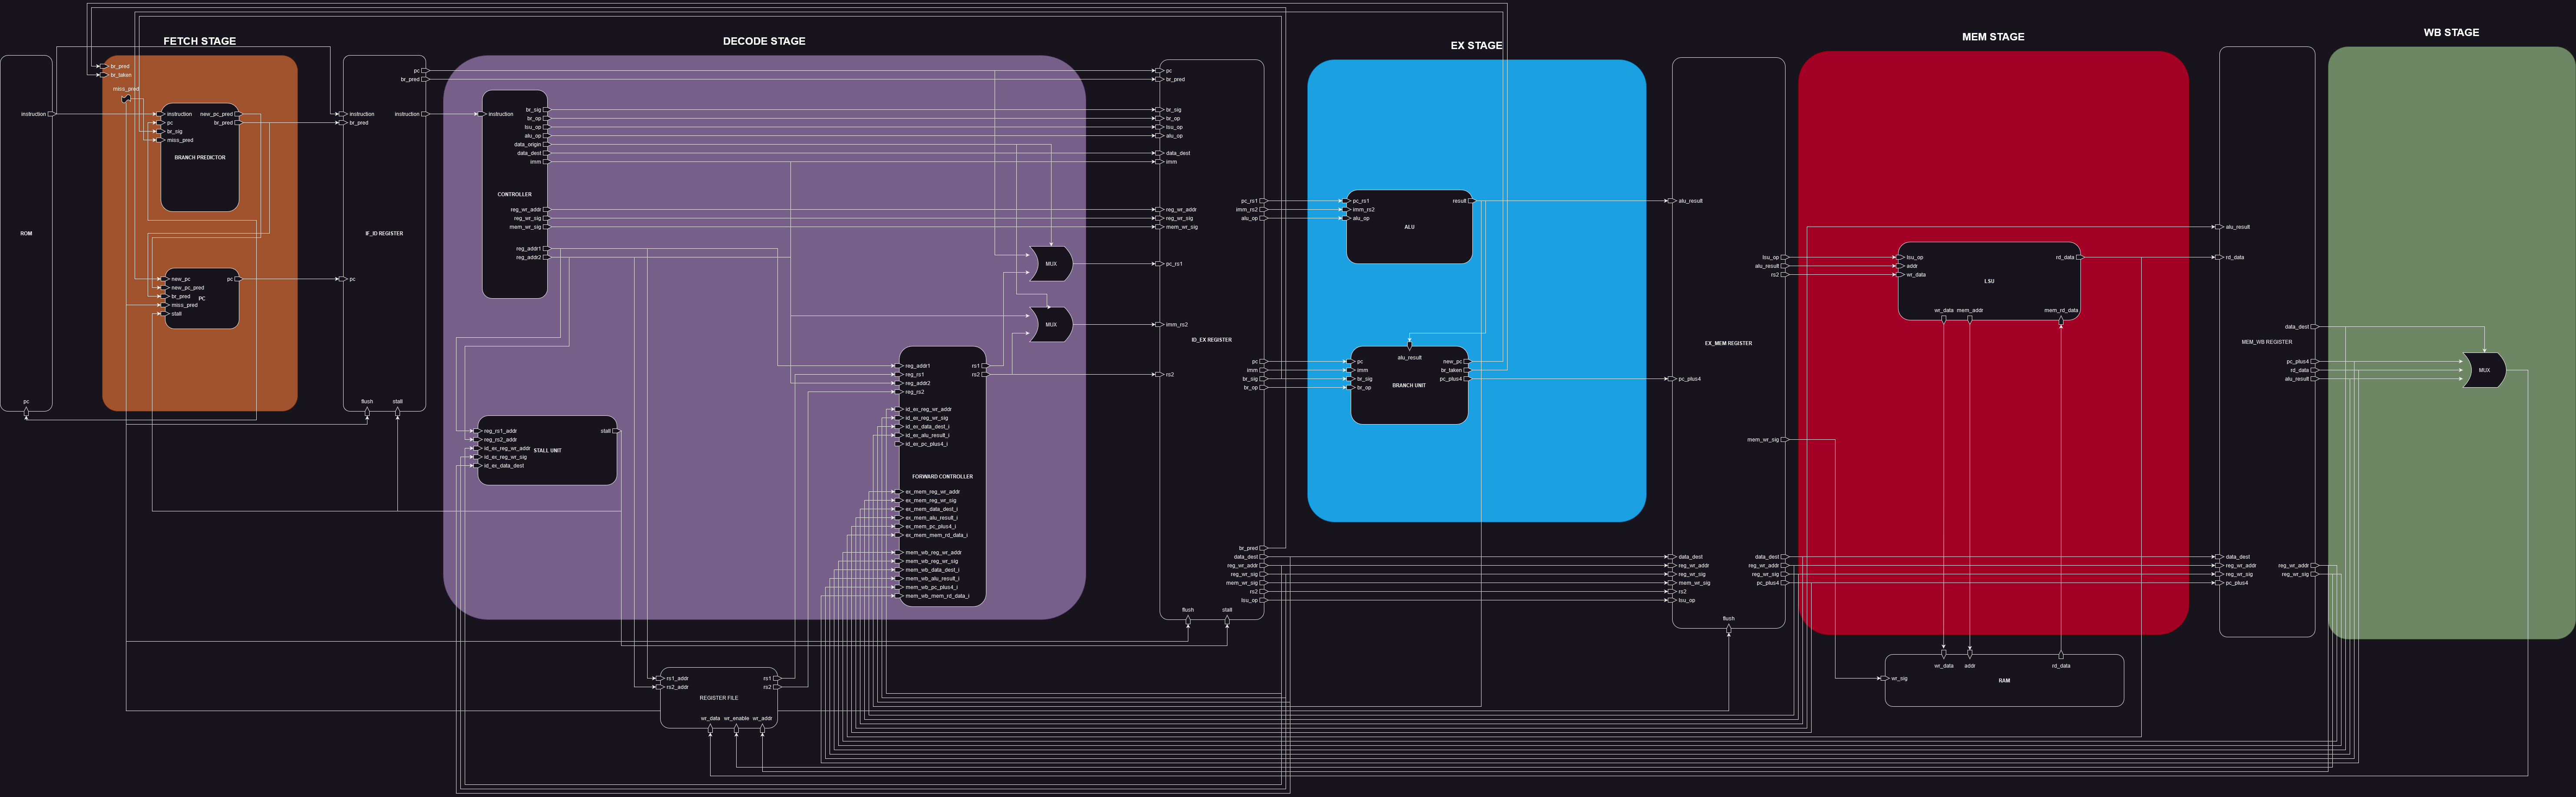
\includegraphics[width=\textheight]{appendix/images/pipelined_design_detail.png} % Note the change in width to \textheight
    \caption{Detailed Pipelined CPU Design}
\end{sidewaysfigure}
\end{document}
